\documentclass[portuguese,oneside]{tcc}

\usepackage{graphicx}
\usepackage{multirow}
\usepackage{nicefrac}
\usepackage{algorithmic}
\usepackage{calc}
\usepackage{enumitem}
\usepackage{tikz}
\usepackage{mdframed}

\usepackage{listings}

\usepackage{subcaption}
\captionsetup{compatibility=false}

\usetikzlibrary{shapes.geometric}
\usetikzlibrary{shapes.misc}
\usetikzlibrary{positioning}
\usetikzlibrary{fit}
\usetikzlibrary{trees}

\author{Martin Duarte Móre e William Henrihque Martins}

\title{Explorando as Cavernas de Spelunky Utilizando Agentes Inteligentes}
      {Exploring Spelunky's Caves Using Intelligent Agents}

\tipotrabalho{\tci}

\curso{\cc}

\orientador{Felipe Meneguzzi}

\begin{document}

%\dedicatoria{Dedico este trabalho a meus pais.}

%\epigrafe{The art of simplicity is a puzzle of complexity.}
%         {Douglas Horton}

%\begin{agradecimentos}
%\end{agradecimentos}

\begin{resumo}{Spelunky, jogo de computador, SpelunkBots, inteligência
artificial, agentes inteligentes}
\textit{Spelunky} é um premiado jogo de computador fácil de aprender, mas
difícil de dominar. O objetivo do jogador é explorar cavernas subterrâneas
enquanto coleta tesouros valiosos. Este trabalho tem como objetivo propor
soluções de Inteligência Artificial para a criação de agentes inteligentes
capazes de jogar com autonomia o jogo \textit{Spelunky}.
\end{resumo}

\begin{abstract}{Spelunky, computer game, SpelunkBots, artificial intelligence,
intelligent agents}
\textit{Spelunky} is an award-winning computer game that is easy to learn, but
hard to master. The player's goal is to explore underground caves whilst
collecting valuable treasures. This work aims to propose Artificial Intelligence
solutions for creating intelligent agents capable of playing autonomously the
game \textit{Spelunky}.
\end{abstract}

\listoffigures
%\listoftables
\listofalgorithms
%\listofacronyms
%\listofabbreviations
%\listofsymbols
\tableofcontents

\chapter{\label{chap:introduction}Introdução}

\sigla{API}{Application Programming Interface}
\sigla{BT}{Behavior Tree}
\sigla{DLL}{Dynamic-link Library}
\sigla{FSM}{Finite-State Machine}
\sigla{GML}{GameMaker Language}
\sigla{HFSM}{Hierarchical Finite-State Machine}
\sigla{NEAT}{Neuroevolution of Augmenting Topologies}
\sigla{TWEANN}{Topology and Weight Evolving Artificial Neural Network}

A popularização dos jogos digitais se deu nas décadas de 70 e 80 com o
surgimento dos computadores pessoais, os fliperamas e os \textit{consoles} de
jogos. Apesar de sofrer uma retração com o \textit{crash} de
83\footnote{Recessão na indústria de jogos digitais que ocorreu de 1983 a 1985.
A principal causa foi a saturação do mercado.}, o mercado de jogos digitais
ascendeu rapidamente. Em 2014, obteve uma receita de aproximadamente 80 bilhões
de
dólares\footnote{https://newzoo.com/insights/articles/top-100-countries-represent-99-6-81-5bn-global-games-market/}.
Isto mostra que os seres humanos possuem um interesse significativo por jogos
digitais. Como consequência, a indústria está em constante aprimoramento,
buscando produzir jogos mais interessantes, inovadores e desafiadores, a fim de
manter seu público alvo e atrair novos jogadores. Um dos aliados dos jogos
digitais para atingir este objetivo é o uso de técnicas sofisticadas de
inteligência artificial para criar conteúdos complexos e engajar ainda mais
os jogadores\cite{PanoramaAIGames}.

Paralelamente, a área de inteligência artificial também se beneficia ao se
relacionar com jogos digitais. Jogos podem ser utilizados como plataformas de
testes para seus algoritmos e técnicas, pois são muito acessíveis, são capazes
de reproduzir cenários reais em ambientes virtuais e seu uso torna o processo
mais barato e rápido que, por exemplo, realizar testes no mundo real com objetos
físicos\footnote{http://togelius.blogspot.com/2016/01/why-videogames-are-essential-for.html}.
Diversas competições de inteligência artificial foram criadas recentemente
utilizando jogos digitais como plataforma de teste\cite{GameAiCompetition}.
Estas competições geralmente possuem como objetivo principal a criação de
agentes inteligentes capazes de jogar o jogo proposto da maneira mais eficiente
possível, seja por pontuação, seja por tempo. Uma destas competições, baseada no
jogo de computador \textit{Spelunky}, se chama \textit{SpelunkBots}. Os
criadores desta competição desenvolveram uma aplicação de inteligência
artificial que facilita a criação de agentes inteligentes para o jogo.

\textit{Spelunky} é um jogo de computador considerado fácil de aprender mas
extremamente difícil de dominar, pois requer que o jogador possua reações
rápidas para perigos iminentes e, ao mesmo tempo, pense em táticas e estratégias
de longo prazo para ser bem-sucedido. Ao todo, são 26 inimigos, 14 armadilhas e
43 itens diferentes\footnote{Dados extraídos da Spelunky Wiki
(http://spelunky.wikia.com/wiki/Spelunky\_Wiki).}. O jogador, ao iniciar uma
partida, sempre se depara com um nível completamente diferente, pois o jogo faz
uso de um algoritmo complexo para gerar níveis. Estes fatores fazem com que
\textit{Spelunky} seja um jogo com desafios interessantes para a pesquisa em
inteligência artificial.

Este trabalho tem como objetivo a construção de agentes inteligentes capazes de
jogar o jogo \textit{Spelunky}, considerado como um problema de difícil solução.
Para tal, utilizaremos o \textit{framework} \textit{SpelunkBots} e
implementaremos as técnicas de inteligência artificial \textit{Behavior Trees} e
\textit{NEAT} em agentes jogadores de \textit{Spelunky}, avaliando e comparando
seus desempenhos e resultados obtidos.

Primeiramente, no capítulo \ref{chap:introduction}, apresentamos uma breve
contextualização da relação entre jogos digitais e inteligência artificial,
nossas motivações para o surgimento deste projeto, uma descrição resumida de
nossos objetivos e um detalhamento da estrutura deste documento. Depois, no
capítulo \ref{chap:spelunky}, examinamos o universo do jogo \textit{Spelunky}.
Em seguida, no capítulo \ref{chap:spelunkbots}, levantaremos alguns pontos
importantes sobre competições de inteligência artificial com base em jogos
digitais e, depois disso, forneceremos uma breve explicação do funcionamento do
\textit{framework} \textit{SpelunkBots}. No capítulo \ref{chap:theory},
estabelecemos a base teórica necessária para compreender as técnicas de
inteligência artificial escolhidas para o desenvolvimento dos \textit{bots}.
Depois, no capítulo \ref{chap:project}, apresentamos uma explicação dos
problemas e objetivos deste trabalho, e depois traçamos os requisitos e detalhes
do projeto de implementação. Por fim, no capítulo \ref{chap:work-plan},
definimos as atividaddes necessárias para atingirmos os objetivos estipulados e
apresentamos um cronograma de execução deste projeto.

\chapter{\label{chap:spelunky}Spelunky}
Spelunky\footnote{http://www.spelunkyworld.com/original.html} é um jogo onde o
jogador incorpora um aventureiro que decide explorar uma caverna misteriosa. O
local contém tesouros, mas também está repleto de perigos. O objetivo principal
do jogador é explorar estas cavernas subterrâneas e coletar a maior quantia de
tesouros possível enquanto evita ser abatido pelos diversos inimigos e
armadilhas espalhadas pelo ambiente.

O jogo se enquadra no gênero \textit{platformer}, estilo de jogo que envolve
guiar um personagem através de plataformas suspensas e obstáculos para obter
progresso no jogo, e é fortemente inspirado em alguns dos elementos-chave do
gênero \textit{roguelike} -- tipo de jogos que se popularizou na década de 80
caracterizados por sua dificuldade, enfoque em exploração de ambientes e
narrativa fantasiosa --, como \textbf{geração procedural} e \textbf{morte
permanente} (Estes elementos são explicados em detalhe nas seções
\ref{section:spelunky-procgen} e \ref{section:spelunky-structure}). A Figura
\ref{fig:spelunky-gameplay} ilustra uma partida do jogo.

\begin{figure}[htb!]
\centering
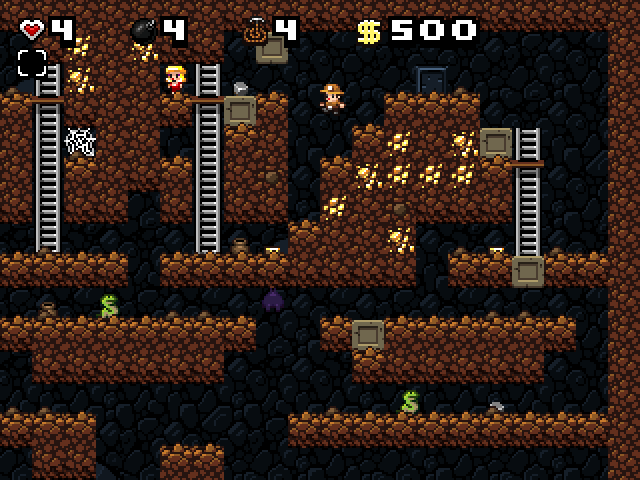
\includegraphics[width=.65\textwidth]{fig/spelunky-pc-screen.png}
\caption{\label{fig:spelunky-gameplay}Exemplo de partida de spelunky, mostrando
elementos do jogo como o jogador, a caverna, os inimigos, os tesouros, entre
outros.}
\end{figure}


%----------
\section{\label{section:spelunky-goals}Objetivos}
Apesar de o \textbf{objetivo principal} em Spelunky ser completar todos os
níveis, o jogo baseia a qualidade das partidas utilizando um sistema de
\textit{high scores}. Para tal, faz uso de uma série de métricas para
classificar os jogadores ao término de uma partida. Estas métricas são:

\begin{itemize}
	\item \textbf{Pontuação:} Mede a quantidade de tesouros obtidos pelo jogador
	no decorrer da partida. Existem diversos tipos de tesouros, como barras de
	ouro, pedras preciosas e estatuetas sagradas. Salvas as estatuetas sagradas,
	que devem ser carregadas até o fim do nível, o jogador precisa simplesmente
	tocar um tesouro para coletá-lo. Os tesouros se encontram espalhados pelo
	chão, dentro do terreno, dentro de baús ou são deixados por certos inimigos
	ao serem abatidos.

	\item \textbf{Tempo:} Mede o tempo para completar a partida. Começa a contar
	a partir do momento em que o jogador entra no primeiro nível e para de
	contar no fim do último nível. A contagem de tempo é interrompida durante as
	transições de nível e quando o jogador pausa a partida.

	\item \textbf{Abates:} Quantidade de inimigos abatidos pelo jogador durante
	a partida. Mortes acidentais de inimigos -- cair de um penhasco, acionar uma
	armadilha, etc. -- não aumentam este contador.

	\item \textbf{Salvamentos:} Quantidade de donzelas em perigo que foram
	resgatadas pelo jogador. Geralmente existe uma donzela em perigo por nível,
	mas existe a possibilidade -- mesmo que pequena -- de uma donzela não
	aparecer em alguns níveis. Para resgatar uma donzela, o jogador deve
	carregá-la com vida até a saída do nível.
\end{itemize}

Embora o jogo ofereça 4 métricas de classificação diferentes, a comunidade de
jogadores de Spelunky não mostra interesse significativo em atingir quantidades
elevadas de número de abates e número de salvamentos, se concentrando apenas em
atingir pontuações máximas e em concluir o jogo no menor tempo
possível\footnote{Comunidade de ranking de jogadores de Spelunky:
https://mosstier.com}. Pode-se concluir, portanto, que os \textbf{objetivos
secundários} mais importantes são a pontuação final e o tempo de partida. A
Figura \ref{fig:spelunky-scores} mostra um exemplo de pontuação final obtida.

\begin{figure}[htb!]
\centering
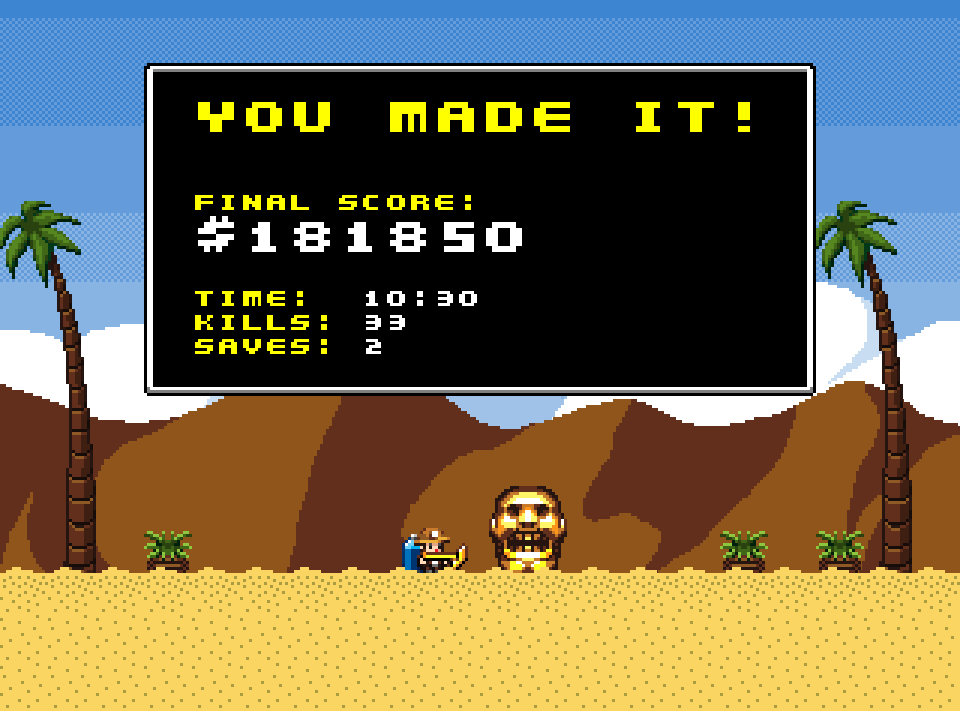
\includegraphics[width=.65\textwidth]{fig/spelunky-score.png}
\caption{\label{fig:spelunky-scores}Exemplo de pontuação final obtida ao fim de
uma partida de Spelunky.}
\end{figure}


%----------
\section{\label{section:spelunky-structure}Estrutura do jogo}
Uma partida de Spelunky é dividida em \textbf{níveis}, cada um sendo
representado por um mapa diferente. O jogador, ao entrar em um nível, é
posicionado na parte superior do mapa. Como não é informado ao jogador a posição
exata da saída, ele deve explorar o ambiente até encontrá-la. A saída sempre
está localizada em algum lugar na parte mais inferior do mapa. Ao utilizar a
saída, o jogador é enviado para o próximo nível e não pode retornar ao mapa que
acabou de completar.

O jogo é dividido em 4 \textbf{áreas} principais: \textbf{As Minas} (níveis 1 a
4), \textbf{A Selva} (níveis 5 a 8), \textbf{As Cavernas de Gelo} (níveis 9 a
12) e \textbf{O Templo} (níveis 13 a 16). Cada área possui um estilo de mapa e
aparência única. A dificuldade do jogo também aumenta gradativamente conforme o
jogador avança pelas áreas, principalmente porque os inimigos vão se tornando
cada vez mais fortes. O último nível do Templo é o \textbf{Covil de Olmec}. onde
o jogador deve enfrentar e derrotar \textbf{Olmec}. Após derrotar o inimigo
final, o explorador é recompensado com uma estatueta gigante feita de ouro e o
jogo termina.


\subsection{Atalhos}
É possível, ao iniciar uma partida, burlar este progresso entre áreas e ir
diretamente para as três ultimas áreas do jogo utilizando atalhos, criados pelo
personagem conhecido como \textbf{Homem do Túnel}. Para ter acesso a estes
atalhos, o jogador deve primeiramente auxiliar o Homem do Túnel a criá-los. O
personagem sempre aparece ao fim do último nível das primeiras três áreas do
jogo -- níveis 4, 8 e 12 --, se oferecendo para criar uma passagem secreta que
leva ao início da área que o jogador está prestes a chegar. Para criar a
passagem, o jogador deve ceder ao Homem do Túnel uma certa quantia de dinheiro.
O atalho da Selva, das Cavernas de Gelo e do Templo custam 100.000, 200.000 e
300.000, respectivamente.

Uma vez construídas, estas passagens são permanentes e podem ser acessadas ao
início de uma partida. Contudo, é importante ressaltar que, ao burlar etapas do
jogo, a pontuação do jogador não será contada para os \textit{high scores}. A
Figura \ref{fig:spelunky-tunnelman} ilustra a construção de um atalho e o acesso
aos atalhos antes do início da partida.

\begin{figure}[htb!]
\centering
	\begin{subfigure}[b]{0.4\textwidth}
		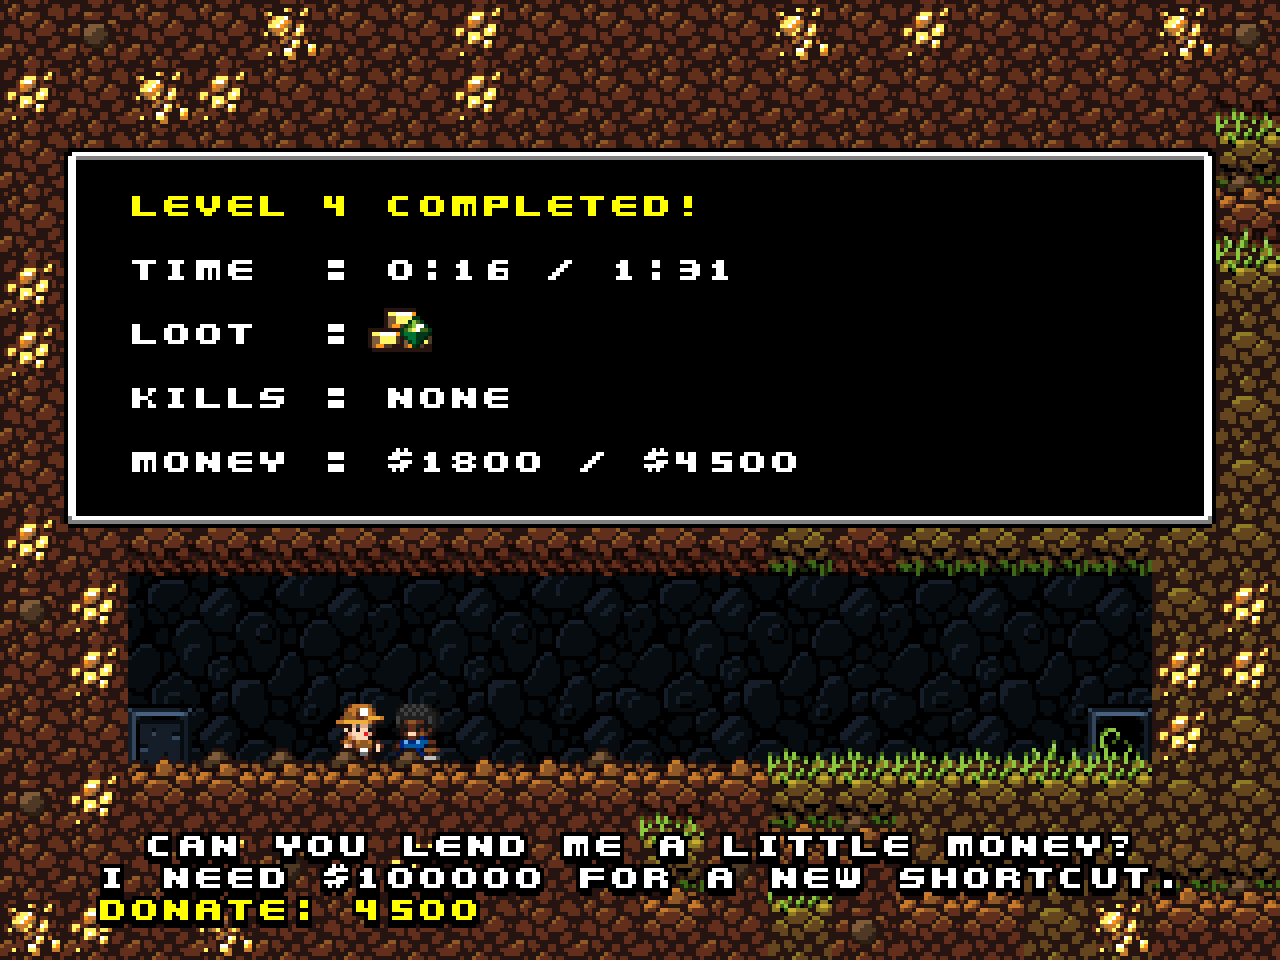
\includegraphics[width=\textwidth]{fig/spelunky-tunnelman.png}
		\caption{O Homem do Túnel solicitano ajuda para construir o atalho para
		a Selva.}
		\label{fig:spelunky-tunnelman}
	\end{subfigure}
	\begin{subfigure}[b]{0.4\textwidth}
		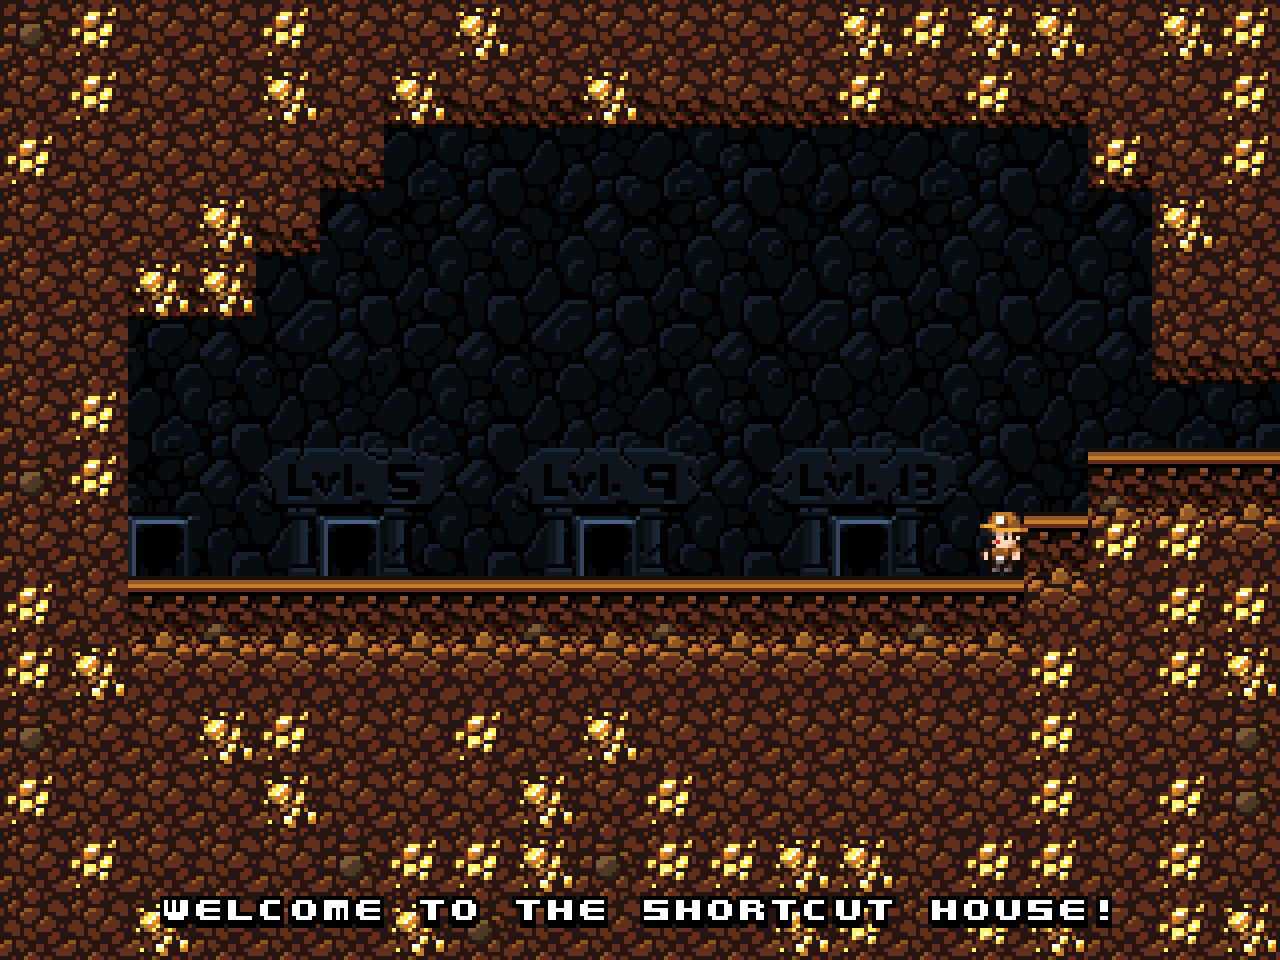
\includegraphics[width=\textwidth]{fig/spelunky-shortcuts.png}
		\caption{Os atalhos disponíveis antes do início da partida.}
		\label{fig:spelunky-shortcuts}
	\end{subfigure}
	\caption{Exemplo das interações com o Homem do Túnel e com os atalhos de
	\textit{Spelunky}.}
	\label{fig:spelunky-shortcuts-example}
\end{figure}


\subsection{Áreas Secretas}
Além das áreas principais, existem duas áreas secretas: \textbf{O Mercado Negro}
e \textbf{A Cidade de Ouro}. Estas áreas do jogo são fundamentais para se obter
equipamentos e grandes quantidadeds de tesouros, mas o jogador só obterá acesso
a elas se respeitar uma série de requisitos impostos pelo jogo. A Figura
\ref{fig:spelunky-secret-areas} exemplifica a aparência destas áreas secretas.

\begin{figure}[htb!]
\centering
	\begin{subfigure}[b]{0.4\textwidth}
		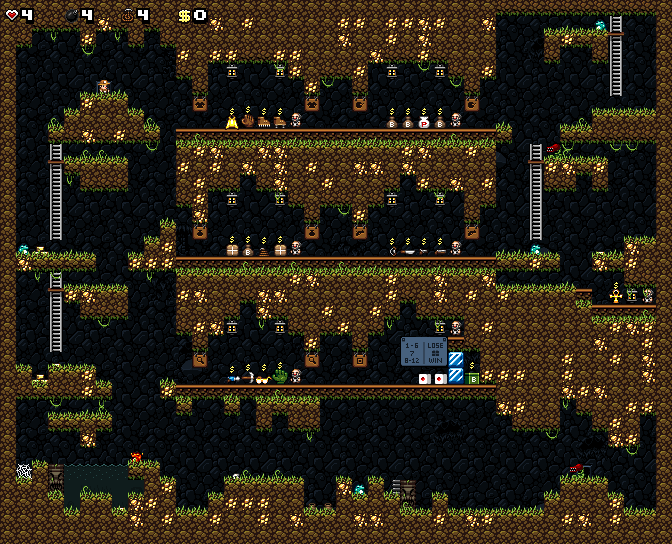
\includegraphics[width=\textwidth]{fig/spelunky-blackmarket.png}
		\caption{O Mercado Negro}
		\label{fig:spelunky-blackmarket}
	\end{subfigure}
	\begin{subfigure}[b]{0.4\textwidth}
		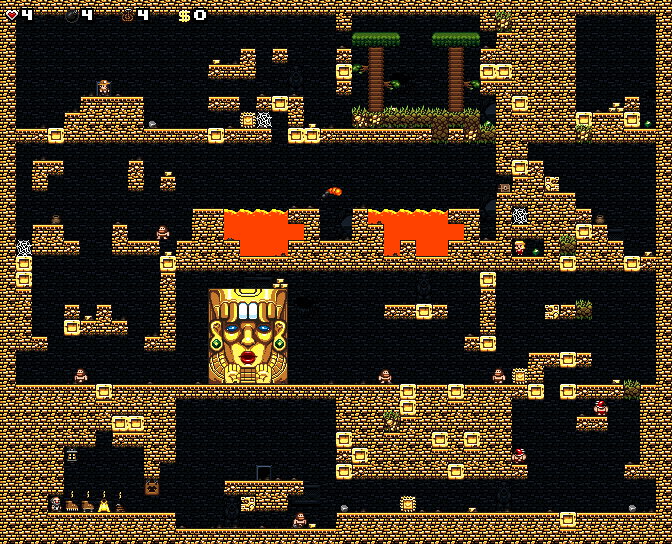
\includegraphics[width=\textwidth]{fig/spelunky-cityofgold.png}
		\caption{A Cidade de Ouro}
		\label{fig:spelunky-cityofgold}
	\end{subfigure}
	\caption{Exemplos das áreas secretas que podem ser acessadas pelo jogador em
	\textit{Spelunky}}
	\label{fig:spelunky-secret-areas}
\end{figure}


Para entrar no Mercado Negro, o jogador deve encontrar sua entrada -- que estará
oculta dentro do terreno do mapa -- enquanto explora a área da selva. O jogador
pode utilizar um item especial chamado \textbf{Udjat Eye} para ajudá-lo a
encontrar a entrada da área. O uso do item não é necessário, mas é aconselhável,
pois é quase impossível de localizar a entrada sem ele. Dentro do mercado negro,
o jogador encontrará vários comerciantes e terá a oportunidade de trocar seus
tesouros por equipamentos e itens diversos.

Entrar na Cidade de Ouro é muito mais complexo e é considerado um dos maiores
desafios do jogo, pois requer que o jogador colete uma série de artefatos
egípcios -- ilustrados na Figura \ref{fig:spelunky-artifacts} -- e execute uma
longa cadeia de ações ao longo da partida. A Cidade de Ouro é idêntica a um
nível do Templo, mas o terreno é feito de ouro maciço -- podendo ser destruído
com bombas -- e contém muito mais tesouros para coletar.  Além disso, o nível
contém uma estátua dourada gigante feita de ouro e pedras preciosas que pode ser
destruída pelo jogador. As etapas para entrar na Cidade de Ouro são:

\begin{enumerate}
	\item Coletar o \textbf{Udjat Eye}: O primeiro artefato se encontra dentro
	de um baú em algum nível da primeira área do jogo, as Minas. O jogador deve
	localizar a chave deste baú -- que se encontra no mesmo nível -- para poder
	abrí-lo. O Udjat Eye é capaz de encontrar a localização exata da entrada do
	Mercado Negro. O artefato pisca e brilha quanto mais próximo da entrada o
	jogador estiver, facilitando a localização da entrada.

	\item Coletar o \textbf{Ankh}: O segundo artefato se encontra no Mercado
	Negro e pode ser comprado (ou furtado) de um comerciante específico que
	vende somente este ítem. O Ankh oferece ao jogador uma segunda vida, caso
	venha a sucumbir.

	\item Coletar o \textbf{Hedjet}: O terceiro artefato pode ser obtido nas
	Cavernas de Gelo. Para obtê-lo, o jogador deve localizar um Moai\footnote{
	Estrutura monolítica com aparência humana. Os Moai foram esculpidos pelos
	Rapa Nui, habitantes nativos da Ilha de Páscoa.} e se morrer próximo a ele.
	O Ankh trará o jogador de volta a vida dentro do Moai e permitirá que o
	jogador colete o Hedjet.

	\item Coletar o \textbf{Cetro}: O quarto e último artefato podde ser obtido
	na última área do jogo, o Templo. O jogador deve encontrar e derrotar a
	Múmia, um dos inimigos mais fortes do jogo. Ao morrer, a múmia deixará o
	Cetro no chão. O Cetro é diferente dos outros itens porque, na verdade, é
	uma arma. Ele solta raios laser de cor rosa em formato de anel que perseguem
	e matam o inimigo mais próximo.

	\item Localizar a \textbf{Porta Dourada}: A última etapa do processo é
	encontrar a entrada da Cidade de Ouro, localizada em algum dos níveis do
	Templo. O jogador deve abandonar o Cetro e utilizá-lo como chave na Porta
	Dourada.
\end{enumerate}

\begin{figure}[htb!]
\centering

\includegraphics[width=.65\textwidth]{fig/spelunky-artifacts.png}
\caption{\label{fig:spelunky-artifacts}Os artefatos místicos de
\textit{Spelunky} necessários para acessar a Cidade de Ouro. Da esquerda para a
direita: o Udjat Eye, o Ankh, o Hedjet e o Cetro.}
\end{figure}

Não é necessário que o jogador acesse as duas áreas secretas do jogo durante uma
partida, mas as quatro áreas principais devem necessáriamente ser visitadas --
salvo quando o jogador fizer uso de um atalho, abrindo mão da validez de sua
pontuação. É importante ressaltar que o jogo conta com o conceito de
\textbf{morte permanente}, que faz com que o jogador, ao ter seus pontos de vida
esgotados, tenha que recomeçar o jogo desde seu início, perdendo todo o
progresso obtido até então.  A Figura \ref{fig:spelunky-run} ilustra a relação
entre as áreas e o progresso de uma partida de Spelunky.

\begin{figure}[htb!]
\centering
\begin{tikzpicture}[
    room/.style={
        regular polygon, regular polygon sides=4,
        draw=black, fill=white,
        text width=4.5em, text centered,
        minimum size=5mm,
        font=\small
    }
]
\matrix(rooms)[row sep=1cm, column sep=1cm]
{
    \node[room] (r1) {As Minas};            &
    \node[room] (r2) {A Selva};             &
    \node[room] (r3) {As Cavernas de Gelo}; &
    \node[room] (r4) {O Templo};            &

    \\
                                            &
    \node[room] (r5) {O Mercado Negro};     &
                                            &
    \node[room] (r6) {A Cidade de Ouro};    &
    \\
};
\draw[->,>=latex] (r1.east) -- (r2.west);
\draw[->,>=latex] (r2.east) -- (r3.west);
\draw[->,>=latex] (r3.east) -- (r4.west);

\draw[->,>=latex] ([xshift=-.5cm]r2.south) -- ([xshift=-.5cm]r5.north);
\draw[->,>=latex] ([xshift=.5cm]r5.north) -- ([xshift=.5cm]r2.south);

\draw[->,>=latex] ([xshift=-.5cm]r4.south) -- ([xshift=-.5cm]r6.north);
\draw[->,>=latex] ([xshift=.5cm]r6.north) -- ([xshift=.5cm]r4.south);
\end{tikzpicture}
\caption{\label{fig:spelunky-run}Relação entre as áreas de Spelunky durante uma
partida do jogo.}
\end{figure}

%----------
\section{\label{section:spelunky-controls}Controle do Personagem}
Os controles básicos em Spelunky são relativamente simples. Para se deslocar
pelo mapa, o jogador pode enviar comandos ao personagem para \textbf{caminhar},
\textbf{correr} e \textbf{pular}. O explorador também pode se \textbf{pendurar}
com as mãos na lateral de uma plataforma e subir e descer escadas. Como a
visibilidade do mapa é limitada a tela, o jogador pode \textbf{mover a câmera}
levemente na vertical ao \textbf{olhar para cima} ou se \textbf{agaixar},
aumentando sua visibilidade do ambiente. O explorador pode \textbf{utilizar
bombas e cordas} para auxiliar no deslocamento pelo nível. As bombas causam uma
explosão que elimina os inimigos e também desobstrui passagens. Já as cordas
permitem que o personagem atinja partes do mapa que não seriam acessíveis ao
pular, por estarem muito elevadas. Existe a possibilidade, também, de
\textbf{comprar itens} e \textbf{realizar apostas} com tesouros nas lojas dos
comerciantes.

A complexidade nos controles de Spelunky surge com a combinação de ações com
objetos, acessórios e equipamentos. O jogador pode \textbf{carregar um
item} em suas mãos e utilizá-lo quando desejar. O efeito depende do item
equipado atualmente. Por exemplo, se estiver carregando uma pedra, ele o
arremessará para longe. Se estiver segurando uma espingarda, ele realizará um
disparo. Os acessórios e equipamentos também modificam o funcionamento de ações.
Alguns acessórios podem fazer com que o personagem pule mais alto ou seja capaz
de se agarrar nas paredes. Portanto, é necessária atenção para os itens
coletados e equipados atualmente pelo explorador.


%----------
\section{\label{section:spelunky-procgen}Algoritmo de Geração Procedural de
Níveis}
Os níveis de Spelunky são gerados proceduralmente, ou seja, utiliza
um algoritmo capaz de gerar automáticamente os elementos que irão compor o
nível. Isto significa que não existe uma maneira de se memorizar estratégias
específicas de um mapa em Spelunky, pois ao início de cada partida o mapa é
gerado de maneira única e os tesouros, itens e obstáculos são dispostos de
maneira diferente, fazendo com que o jogador tenha que aprender a lidar com os
elementos do jogo de forma individual, combinar este conhecimento e estabelecer
uma estratégia para vencer seus obstáculos e ser bem sucedido.

O algoritmo de geração procedural de níveis de Spelunky é dividido em três
etapas: a \textbf{geração do caminho de solução}, a \textbf{geração de salas} e
a \textbf{disposição de entidades}.

\subsection{\label{section:spelunky-procgen-path}Geração do Caminho de Solução}
Cada nível em Spelunky é construído a partir de 16 \textbf{salas}, dispostas em
uma grade 4 por 4. Nesta etapa do algoritmo é escolhido o \textbf{caminho
solução} do nível, uma sequência de salas que formam um caminho desobstruído da
entrada até a saída. Primeiramente, o gerador escolhe uma das quatro salas da
parte superior para colocar a entrada do nível. Escolhido o local da entrada, o
algoritmo gera um caminho até a saída através de movimentos aleatórios para a
esquerda, para a direita e para baixo na grade de salas. Caso o gerador atinja
um dos extremos horizontais da grade, ele se desloca para baixo e inverte a
direção horizontal do movimento anterior. A saída do nível é colocada quando o
algoritmo chega na última linha da grade e tenta realizar um movimento para
baixo. Assim, a saída sempre se encontrará em uma das quatro salas da parte
inferior do mapa.

Todas as salas que fazem parte do caminho solução são transponíveis do início ao
fim sem o uso de bombas, cordas ou outros equipamentos. Além disso, sempre
possuem aberturas na esquerda e na direita. As salas em que o caminho realiza
uma descida possuem aberturas embaixo e as salas onde o caminho chega de uma
descida possuem aberturas em cima. Isto garante que haverá conectividade entre
todas as salas do caminho principal. Já as salas que não fazem parte do caminho
solução não possuem esta garantia, podendo ser completamente seladas e somente
acessíveis utilizando algum equipamento ou destruindo parte do terreno. Estas
salas fora do caminho solução também podem ser lojas, altares de sacrifício,
altares de ídolos dourados, entre outras. A Figura
\ref{fig:spelunky-procgen-path} exemplifica um resultado desta etapa do
algoritmo.

\begin{figure}[htb!]
\centering
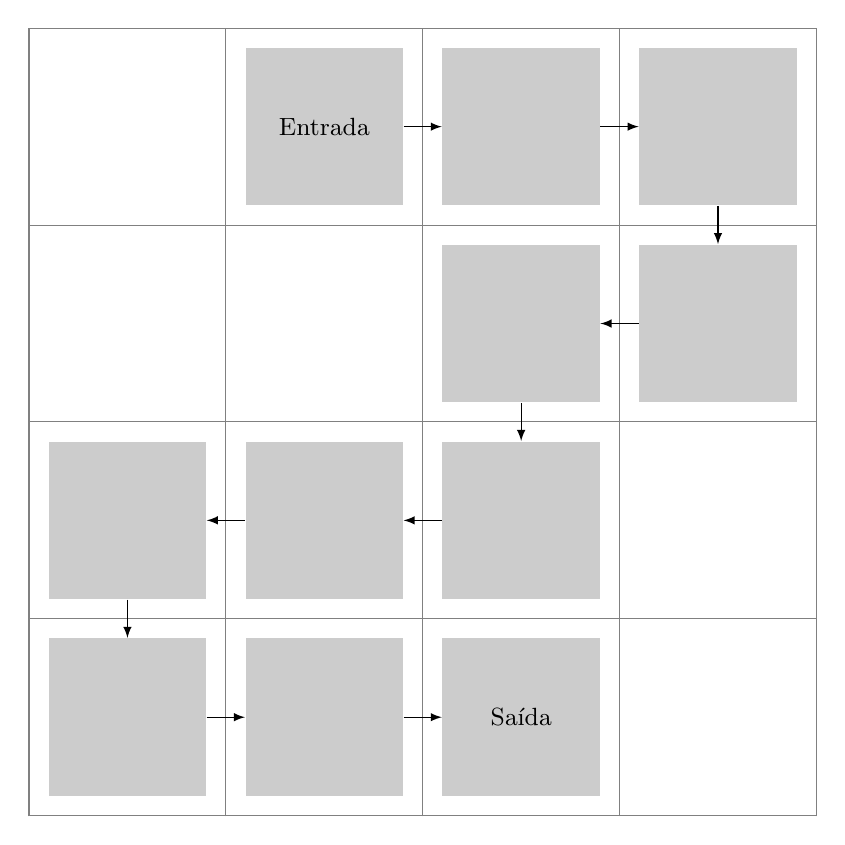
\begin{tikzpicture}[
    box/.style={
        rectangle,
        minimum width={2cm},
        minimum height={2cm},
        fill=gray!40,
        font=\small
    }
]
\draw[step=2.5cm, color=gray] (-5.01, -5.01) grid (5, 5);
\node [box] (b1) at ([xshift=1.25cm,yshift=-1.25cm]-2.5, 5) {Entrada};
\node [box] (b2) at ([xshift=1.25cm,yshift=-1.25cm]0, 5) {};
\node [box] (b3) at ([xshift=1.25cm,yshift=-1.25cm]2.5, 5) {};

\node [box] (b4) at ([xshift=1.25cm,yshift=-1.25cm]2.5, 2.5) {};
\node [box] (b5) at ([xshift=1.25cm,yshift=-1.25cm]0, 2.5) {};

\node [box] (b6) at ([xshift=1.25cm,yshift=-1.25cm]0, 0) {};
\node [box] (b7) at ([xshift=1.25cm,yshift=-1.25cm]-2.5, 0) {};
\node [box] (b8) at ([xshift=1.25cm,yshift=-1.25cm]-5, 0) {};

\node [box] (b9) at ([xshift=1.25cm,yshift=-1.25cm]-5, -2.5) {};
\node [box] (b10) at ([xshift=1.25cm,yshift=-1.25cm]-2.5, -2.5) {};
\node [box] (b11) at ([xshift=1.25cm,yshift=-1.25cm]0, -2.5) {Saída};

\draw[->,>=latex] (b1.east) -- (b2.west);
\draw[->,>=latex] (b2.east) -- (b3.west);

\draw[->,>=latex] (b3.south) -- (b4.north);
\draw[->,>=latex] (b4.west) -- (b5.east);
\draw[->,>=latex] (b5.south) -- (b6.north);

\draw[->,>=latex] (b6.west) -- (b7.east);
\draw[->,>=latex] (b7.west) -- (b8.east);
\draw[->,>=latex] (b8.south) -- (b9.north);
\draw[->,>=latex] (b9.east) -- (b10.west);

\draw[->,>=latex] (b10.east) -- (b11.west);
\end{tikzpicture}
\caption{\label{fig:spelunky-procgen-path}Exemplo de caminho solução gerado na
primeira etapa do algoritmo de geração procedural de níveis de Spelunky.}
\end{figure}

\subsection{\label{section:spelunky-procgen-rooms}Geração de Salas}
A próxima etapa do algoritmo é gerar separadamente as salas que irão compor o
nível. Para fazer isto, o gerador se baseia em \textit{layouts} de salas
pré-estabelecidos pelo desenvolvedor, sendo que cada tipo possui em torno de 6 a
12 \textbf{modelos}. Estes modelos são descritos através de sequências de
caracteres comuns. Uma sala em Spelunky é representada por uma grade 10 por 8 de
\textit{tiles}\footnote{Tipo de representação visual muito utilizada por jogos
2D para dispor os elementos de um jogo em forma de grade, onde cada elemento se
chama \textit{tile}.}, o que significa que cada modelo deve conter exatamente 80
caracteres. A Figura \ref{fig:spelunky-procgen-room-template} ilustra um exemplo
de modelo utilizado pelo gerador.

\begin{figure}[htb!]
\centering
\begin{tabular}{c c c c c c c c c c}
    0 & 0 & 0 & 0 & 0 & 0 & 0 & 0 & 1 & 1 \\
    0 & 0 & 6 & 0 & 0 & 0 & 0 & L & 0 & 4 \\
    0 & 0 & 0 & 0 & 0 & 0 & 0 & P & 1 & 1 \\
    0 & 0 & 0 & 0 & 0 & 0 & 0 & L & 1 & 1 \\
    0 & 0 & 0 & 0 & 0 & 0 & 0 & L & 1 & 1 \\
    0 & 0 & 0 & 0 & 0 & 0 & 0 & 0 & 1 & 1 \\
    0 & 0 & 0 & 0 & 0 & 0 & 0 & 0 & 1 & 1 \\
    1 & 1 & 1 & 1 & 1 & 1 & 1 & 1 & 1 & 1 \\
\end{tabular}
\caption{\label{fig:spelunky-procgen-room-template}Exemplo de modelo utilizado
para gerar uma sala de Spelunky.}
\end{figure}

Cada caractere possui um significado diferente, informando ao gerador que tipo
de \textit{tile} deve ser utilizado em sua posição. Eles podem ser
\textbf{estáticos} ou \textbf{probabilísticos}. Os estáticos sempre são
substituídos pelo seu \textit{tile} correspondente. Os caracteres ``1'' (bloco
sólido), ``L'' (escada) e ``P'' (escada com plataforma) são exemplos deste
tipo. Já os probabilísticos possuem uma chance de serem substituídos pelo seu
\textit{tile} correspondente ou por um espaço vazio. Os caracteres ``2'' (50\%
de chance de ocorrer um bloco sólido) e ``4'' (25\% de chance de ocorrer um
bloco de empurrar) são exemplos do segundo tipo.

Os caracteres ``5'' e ``6'' possuem uma característica especial. Eles não são
mapeados para um único \textit{tile}, e sim para um conjunto 5 por 3 de
\textit{tiles}, chamados de \textbf{obstáculos}. Estes conjuntos também utilizam
sequências de caracteres pré-definidos para descrever seu \textit{layout}.
Existem dois tipos de conjuntos, os aéreos e os terrestres. A diferença entre os
tipos de conjunto é simples: um conjunto terrestre deve ser colocado próximo ao
chão e um conjunto aéreo deve ser colocado no ar. Quando o gerador está
realizando a montagem da sala e detecta um caractere de obstáculo, ele realiza
uma substituição por um dos modelos disponíveis. A Figura
\ref{fig:spelunky-procgen-room-chunk} exemplifica um modelo de obstáculos.

\begin{figure}[htb!]
\centering
\begin{tabular}{c c c c c}
    0 & 1 & 1 & 1 & 0 \\
    0 & 2 & 2 & 2 & 0 \\
    0 & 0 & 0 & 0 & 0
\end{tabular}
\caption{\label{fig:spelunky-procgen-room-chunk}Exemplo de modelo de conjunto de
\textit{tiles} utilizado para gerar uma sala de Spelunky.}
\end{figure}

O uso destes conjuntos ajuda a aumentar a aleatoriedade dos \textit{layouts} das
salas, trazendo a sensação de uma variedade maior, mesmo que o número de modelos
de salas seja pequeno. O resultado da combinação do modelo da sala da
representada na Figura \ref{fig:spelunky-procgen-room-template} com o modelo de
obstáculos representado na Figura \ref{fig:spelunky-procgen-room-chunk} é
evidenciado na Figura \ref{fig:spelunky-procgen-room-combination}.

\begin{figure}[htb!]
\centering
\begin{tabular}{c c c c c c c c c c}
    0 & 0 & 0 & 0 & 0 & 0 & 0 & 0 & 1 & 1 \\
    0 & 0 & 0 & 1 & 1 & 1 & 0 & L & 0 & 4 \\
    0 & 0 & 0 & 2 & 2 & 2 & 0 & P & 1 & 1 \\
    0 & 0 & 0 & 0 & 0 & 0 & 0 & L & 1 & 1 \\
    0 & 0 & 0 & 0 & 0 & 0 & 0 & L & 1 & 1 \\
    0 & 0 & 0 & 0 & 0 & 0 & 0 & 0 & 1 & 1 \\
    0 & 0 & 0 & 0 & 0 & 0 & 0 & 0 & 1 & 1 \\
    1 & 1 & 1 & 1 & 1 & 1 & 1 & 1 & 1 & 1 \\
\end{tabular}
\caption{\label{fig:spelunky-procgen-room-combination}Exemplo de um modelo de
sala e um modelo de conjunto de \textit{tiles} utilizados para gerar uma sala de
Spelunky.}
\end{figure}

Com a descrição dos caracteres em mão, podemos realizar uma interpretação do
modelo ilustrado na Figura \ref{fig:spelunky-procgen-room-combination}. O modelo
descreve uma sala com chão, uma parede à direita, uma escada que leva a uma
pequena passagem, obstruída por um bloco de empurrar, e alguns blocos aéreos que
o jogador pode utilizar para se movimentar.

\subsection{\label{section:spelunky-procgen-entities}Disposição de Entidades}
A última etapa do algoritmo envolve a disposição dos inimigos, tesouros e
armadilhas. O algoritmo percorre todos os \textit{tiles} sólidos do nível a fim
de decidir se colocará uma entidade naquele local ou em suas proximidades.  Cada
tipo de entidade possui restrições diferentes:

\begin{description}
	\item[Inimigos]
	necessitam de espaços vazios acima ou abaixo do \textit{tile} sendo
	verificado atualmente. Inimigos não são colocados em locais muito apertados,
	dentro da água ou dentro da sala que contém a entrada do nível.

	\item[Tesouros]
	podem ser gerados acima de qualquer \textit{tile} sólido, mas a chance e
	valor do tesouro aumentam para locais apertados e em buracos no chão. Não
	são gerados perto da entrada e da saída.

	\item[Armadilhas]
	os requisitos variam muito de acordo com o tipo de armadilha, que podem ser
	espinhos, lança-flechas, pedregulhos, entre outros.
\end{description}

Cada entidade possui uma chance diferente de ocorrer a cada verificação, e as
probabilidades de ocorrência variam para cada área do jogo. Por exemplo, para
cada \textit{tile} na área das Cavernas, um morcego possui uma chance de 1.66\%
de ser gerado e um homem das cavernas possui uma chance de 0.12\% de ser gerado.
O algoritmo busca, através destas porcentagens, garantir que algumas entidades
apareçam mais frequentemente que outras, balanceando a dificuldade do jogo.

A Figura \ref{fig:spelunky-procgen-examples} exemplifica alguns níveis gerados
pelo algoritmo.

\begin{figure}[htb!]
\centering
	\begin{subfigure}[b]{0.4\textwidth}
		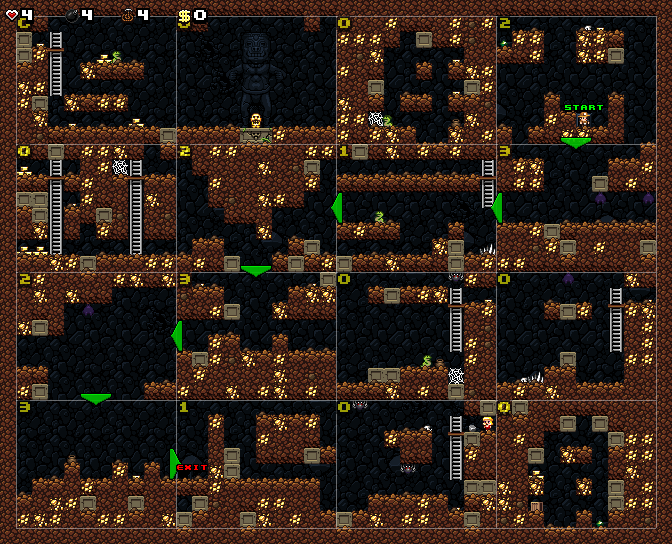
\includegraphics[width=\textwidth]{fig/spelunky-mines-example.png}
		\caption{As Minas}
		\label{fig:spelunky-mines-example}
	\end{subfigure}
	\begin{subfigure}[b]{0.4\textwidth}
		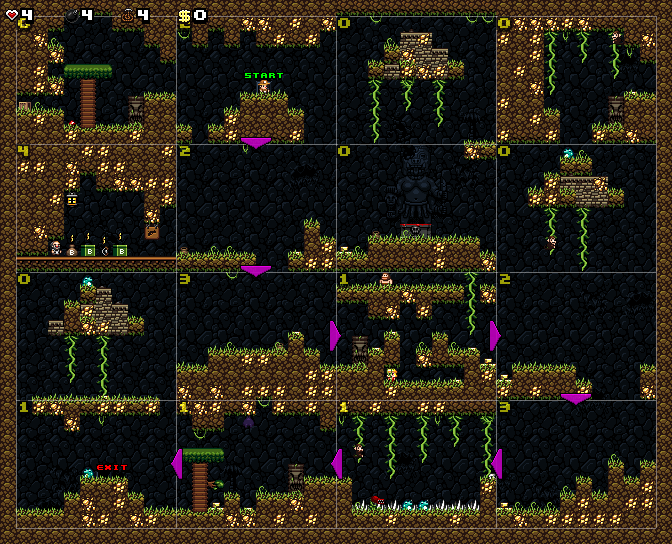
\includegraphics[width=\textwidth]{fig/spelunky-jungle-example.png}
		\caption{A Selva}
		\label{fig:spelunky-jungle-example}
	\end{subfigure}

	\begin{subfigure}[b]{0.4\textwidth}
		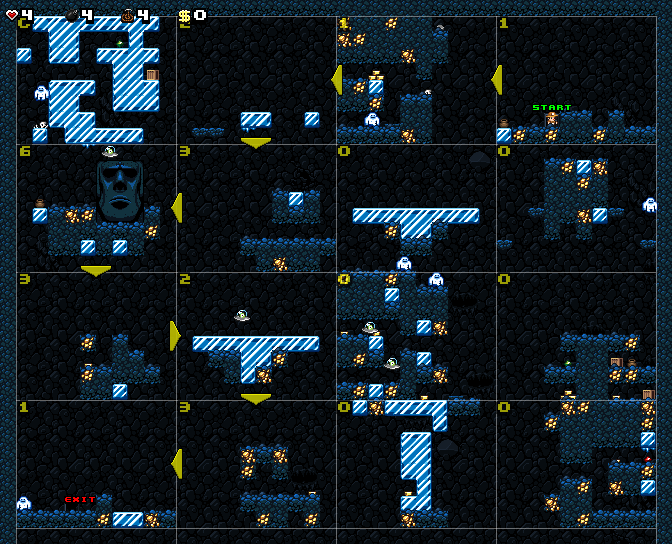
\includegraphics[width=\textwidth]{fig/spelunky-ice-example.png}
		\caption{As Cavernas de Gelo}
		\label{fig:spelunky-ice-example2}
	\end{subfigure}
	\begin{subfigure}[b]{0.4\textwidth}
		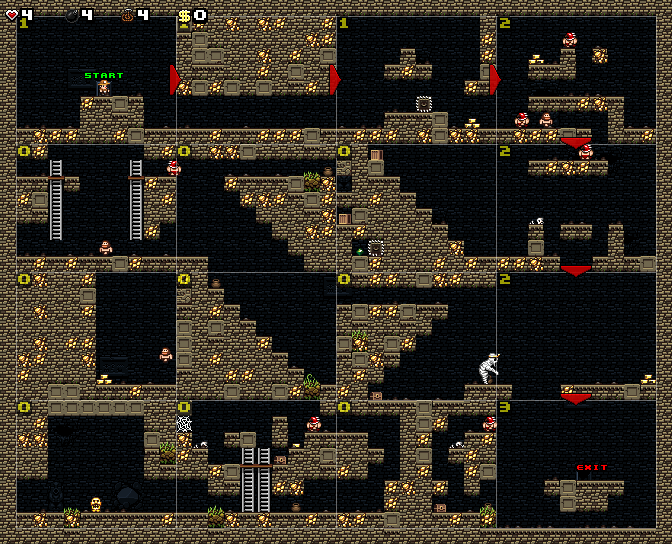
\includegraphics[width=\textwidth]{fig/spelunky-temple-example.png}
		\caption{O Templo}
		\label{fig:spelunky-temple-example}
	\end{subfigure}
	\caption{Exemplos do resultado final do algoritmo de geração de níves de
	\textit{Spelunky} para cada uma das áreas principais do jogo, com
	visualização da entrada, saída e caminho solução.}
	\label{fig:spelunky-procgen-examples}
\end{figure}


%----------
\section{\label{section:spelunky-obstacles}Obstáculos}
O universo de Spelunky é repleto de obstáculos, cujo único objetivo é impedir
que o jogador saia vivo de dentro das cavernas que está explorando. Estes
obstáculos podem ser \textbf{armadilhas} ou \textbf{monstros}. As armadilhas
são objetos projetados para punir invasores indesejados e os monstros são os
habitantes da caverna. Existem diversos tipos de armadilhas e monstros, e
alguns destes inclusive causam a morte instantânea do jogador. O anexo
\ref{section:spelunky-obstacles} apresenta a relação de monstros e
armadilhas, bem como uma breve descrição de seus comportamentos.

Além das armadilhas e monstros, o jogador também deve ter cuidado com os perigos
naturais presentes na caverna, como poços de lava e quedas de lugares muito
altos, pois também pode ser ferido por eles.


%----------
\section{\label{section:spelunky-items}Itens}
Em \textit{Spelunky}, existem diversos objetos com os quais o jogador pode
interagir para obter algum tipo de vantagem durante uma partida. Ao todo, são 43
itens diferentes, que são divididos nas seguintes categorias:

\begin{description}
	\item[Consumíveis]
	Objetos coletados pelo jogador que podem ser utilizados somente uma vez. Em
	alguns casos, o jogador pode carregar mais de um item consumível consigo.
	Alguns exemplo são as bombas, as cordas e o pára-quedas.

	\item[Acessórios]
	Equipamentos que, uma vez coletados pelo jogador, ficam disponíveis para uso
	durante toda a partida. Cada acessório oferece uma habilidade única que
	aumenta as chances de sobrevivência do explorador, e seus efeitos são
	manifestados ou passivamente -- sempre estão ativos -- ou através de uma
	ativação por parte do jogador. Alguns exemplos são o compasso, os sapatos de
	mola e a capa.

	\item[Armas]
	Equipamentos de combate de curto ou longo alcance carregados pelo explorador
	que o auxiliam a enfrentar os diversos monstros presentes na caverna. O
	jogador pode utilizar somente uma arma por vez, pois deve carregar a arma em
	suas mãos para utilizá-la. As armas não podem ser arremessadas pelo jogador.
	Alguns exemplos são o chicote, a espingarda e o arco.

	\item[Diversos]
	Objetos espalhados pela caverna que podem ser carregados e arremessados pelo
	jogador. Muitas vezes, servem como armas improvisadas, pois causam dano ao
	serem arremessadas e colidirem com algum inimigo. Também são utilizados para
	ativar armadilhas, impedindo que o jogador corra o risco de ativá-las sem
	querer. Alguns exemplos são as pedras, os vasos, as caixas e até mesmo
	corpos de inimigos abatidos. 
\end{description}

O anexo \ref{section:spelunky-obstacles} apresenta a relação de itens presentes
em \textit{Spelunky}, bem como uma breve descrição de seus comportamentos.


%----------
\section{\label{section:spelunky-dev}Desenvolvimento e Distribuição}
O jogo foi desenvolvido por Derek Yu -- utilizando o motor de desenvolvimento de
jogos \textit{GameMaker} (Versão 8.0 Pro) -- e lançado gratuitamente para a
plataforma \textit{Windows} em dezembro de
2008\footnote{https://forums.tigsource.com/index.php?topic=4017}. No fim de
2009, o criador optou por liberar o código fonte do jogo, permitindo sua
distribuição não-comercial e
modificação\footnote{http://www.spelunkyworld.com/files/COPYING.txt}. A
liberação do código fonte de Spelunky deve ser considerada um marco muito
importante, pois permitiu a criação de modificações para o jogo. Estas
modificações, normalmente encontradas no fórum oficial da
\textit{Mossmouth}\footnote{http://mossmouth.com/forums/index.php} -- empresa
desenvolvedora de jogos criada por Derek Yu --, são correções de \textit{bugs},
mapas customizados ou até mesmo modos de jogo completamente diferentes do jogo
original. Pode-se dizer que dar esta liberdade para a comunidade do jogo é um
dos fatores que ajuda a manter sua base de jogadores e atraem novos jogadores
até hoje.

O motor GameMaker disponibiliza diversas ferramentas que facilitam o trabalho
do desenvolvedor. Contando com funcionalidades como editores de
\textit{scripts}\footnote{Código desenvolvido para o controle dos
comportamentos dos elementos do jogo.} e de \textit{sprites}\footnote{Elementos
visuais do jogo, tais como o personagem, o fundo, os inimigos. Representados
como uma ou mais imagens, permitindo que as mesmas sejam animadas.},
gerenciadores de eventos, entre
outras\footnote{http://sandbox.yoyogames.com/downloads/docs/gmaker80.pdf}, o
GameMaker oferece um ótimo suporte ao desenvolvedor para a criação de jogos. O
motor disponibiliza uma linguagem de programação própria para seus
\textit{scripts}, a \textit{GameMaker Language}, ou \textit{GML}.

Em julho de 2012, a desenvolvedora \textit{Mossmouth} de Derek Yu lançou uma
versão remasterizada de \textit{Spelunky} para a plataforma \textit{Xbox 360},
nomeada \textit{Spelunky HD}. Esta nova versão possui ainda mais conteúdo que o
original, como novas áreas, monstros, itens, entre outros. Devido ao seu grande
sucesso, esta versão também foi posteriormente lançada para as plataformas
\textit{Windows}, \textit{PlayStation 3} e \textit{PlayStation Vita}. Este
trabalho, contudo, é focado na versão original de \textit{Spelunky}, também
conhecida como \textit{Spelunky Classic}.

\chapter{\label{chap:spelunkbots}SpelunkBots}

\begin{mdframed}[backgroundcolor=green!20]
\begin{itemize}
    \item
        Detalhar mais as informações recebidas pela API
    \item
        Listar e detalhar métodos da API
\end{itemize}
\end{mdframed}

Utilizando o código-fonte de Spelunky, Daniel Scales e Thomas Thompson, da
Universidade de Derby no Reino Unido, criaram o
\textit{SpelunkBots}\cite{SPELUNKBOTSPAPER}, um
\textit{framework} que permite a programação de \textit{bots} para o jogo
Spelunky. Um dos objetivos dos criadores é utilizar a aplicação para criar uma
competição de inteligência artificial para o jogo.

A \textit{API} possibilita que o desenvolvedor resgate informações de objetos
estáticos e dinâmicos contidos no ambiente do jogo, como o terreno, a
posição de tesouros, armadilhas e inimigos. Contudo, o objetivo da \textit{API}
disponibilizada por SpelunkBots é fazer com que a informação recebida pelo
\textit{bot} se assemelhe ao máximo com a percepção de um jogador humano.  Para
tal, o \textit{framework} implementa um sistema de \textit{fog of war},
limitando o conhecimento do ambiente que pode ser obtido pela inteligência
artificial. Para objetos estáticos, uma vez que o jogador visualizou o objeto,
ele poderá receber informações sobre ele permanentemente. Para objetos
dinâmicos, o \textit{bot} só poderá receber informações sobre eles se os mesmos
estiverem sendo visualizados por ele. A figura \ref{fig:spelunkbots-fow} ilustra
um exemplo de funcionamento do sistema, onde as áreas marcadas com o valor ``0''
representam um terreno transponível, enquanto as áreas com o valor ``1''
representam terreno intransponível. As áreas intransponíveis com o fundo
acinzentado correspondem ao sistema de \textit{fog of war}, cujas informações
não estão disponíveis pois tal área ainda não foi explorada pelo \textit{bot}.

\begin{figure}[htb!]
\centering
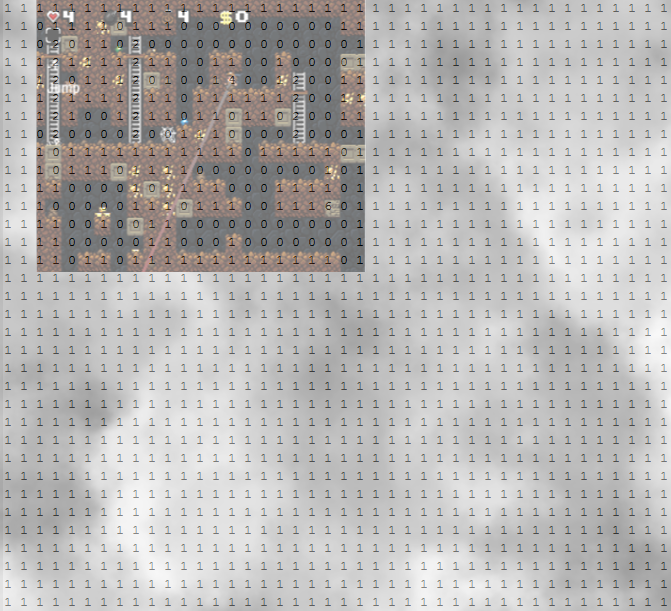
\includegraphics[width=.65\textwidth]{fig/spelunkbots-fow.png}
\caption {\label{fig:spelunkbots-fow}Visualização do sistema de \textit{fog of
war} demonstrando a diferença de informação recebida de elementos dentro e fora
do campo de visão do jogador.}
\end{figure}

\section{Utilização da \textit{API}}

É possível desenvolver \textit{bots} que fazem uso da \textit{API}
utilizando a linguagem GML (sigla para \textit{Game Maker Language}) ou
através da linguagem C++, ficando a critério do desenvolvedor a escolha da
linguagem. A única restrição que existe quanto ao uso de C++ dá-se no fato
de que a linguagem necessita de um processo de compilação através de uma
ferramenta externa, não sendo gerenciada diretamente pelo \textit{Game
Maker}. A figura \ref{fig:spelunkbots-usage-diagram} mostra a relação entre
o jogo, a \textit{API} e as possíveis linguagens de programação para se
utilizar. O código do Spelunky teve de ser modificado de forma a poder
interagir com o código do SpelunkyBots que, por sua vez, faz o uso de uma
solução de \textit{DLLs} escritas em C++ para fazer a interação com o jogo
através de código escrito em C++.

\begin{figure}[htb!]
\centering
\includegraphics[width=.65\textwidth]{fig/spelunkbots-usage-diagram.png}
\caption {\label{fig:spelunkbots-usage-diagram}Diagrama exibindo a relação
entre o jogo Spelunky, a API SpelunkyBots e as linguagens de programação que
podem ser usadas para a interação com o jogo.}
\end{figure}

A \textit{API} permite uma interação completa com o jogo através do uso
das variáveis expostas pelo
\textit{framework}\footnote{http://spelunkbots.com/wp-content/uploads/2015/02/SpelunkBots-API-A-Getting-Started-Tutorial.pdf}.
Com elas, é possível fazer o controle da movimentação do bot, bem
como identificar o tipo de terreno em que se está pisando e os inimigos que
aparecem em seu campo de visão. Além disso, também são disponibilizadas
informações sobre as armadilhas que podem atrapalhar o jogador. Por fim,
existem variáveis que permitem um melhor controle das informações relativas ao
\textit{bot}, como o posicionamento no eixo X e no eixo Y, se o \textit{bot}
encontra-se virado para a esquerda ou para a direita, entre outros. O uso dessas
variáveis torna possível a implementação de técnicas de inteligência artificial
no jogo Spelunky. O apêndice \ref{appendix:spelunkbots-variables} faz um
detalhamento maior de todas essas variáveis.

\chapter{\label{chap:theory}Fundamentação Teórica}
Neste capítulo, apresentaremos a base teórica necessária para compreender o
funcionamento das técnicas \textit{Behavior Trees} e \textit{NEAT}, escolhidas
para realizar o desenvolvimento dos agentes inteligentes de \textit{Spelunky}.

\begin{mdframed}[backgroundcolor=green!20]
\begin{itemize}
	\item
		Explicar a escolha das técnicas
\end{itemize}
\end{mdframed}


%----------
\section{\label{section:environment}Ambientes}
Todas as percepções e ações executadas por agentes racionais ocorrem no
\textbf{ambiente} no qual ele está inserido. A quantidade e variedade de
ambientes encontrados é vasta, mas é possível identificar dimensões (ou
características) de classificação para realizar uma categorização destes
ambientes. Estas características irão determinar que tipos de agentes --
enumerados na seção \ref{section:agents} -- são apropriados para cada ambiente.
As dimensões utilizadas para categorizar ambientes são:

\begin{description}
	\item[Observável, Parcialmente Observável ou Não-Observável]
		Um ambiente é observável se os sensores do agente lhe permitirem acesso
		completo ao estado do ambiente a cada ponto no tempo. Ambientes
		observáveis são convenientes, pois o agente não precisa manter um estado
		interno de conhecimento para se manter informado. O ambiente é
		parcialmente observável se os sensores do agente possuirem ruído ou não
		tiverem acesso completo ao ambiente. Se o agente não possuir nenhum tipo
		de sensor, então o ambiente é não-observável.

	\item[Agente Único ou Multi-Agente]
		Quando o agente não precisa interagir com nenhum outro agente no
		ambiente, então trata-se de um ambiente com agente único. Caso ele
		precise interagir de alguma forma (competição, cooperação ou
		comunicação) com outros agentes, então o ambiente é multi-agente.

	\item[Determinístico ou Estocástico]
		Se o próximo estado do ambiente for completamente determinado pela
		combinação do estado atual com uma ação executada pelo agente, então o
		ambiente é determinístico. Caso contrário, é estocástico.

	\item[Episódico ou Sequencial]
		Em ambientes episódicos, a experiência do agente é dividida em episódios
		atômicos, ou seja, são independentes entre sí. O agente não precisa
		pensar adiante pois, a cada episódio, recebe informações sensoriais e
		executa apenas uma ação, e o próximo episódio não será influenciado pela
		ação anterior. Já em ambientes sequenciais, a ação atual pode
		influenciar todas as decisões futuras, ou seja, ações a curto prazo
		podem ter consequências a longo prazo.

	\item[Discreto ou Contínuo]
		Ambientes discretos são aqueles onde se tem um número contável de ações
		e percepções possíveis. Em ambientes contínuos, o número de ações e de
		percepções muitas vezes são baseados em valores contínuos ou não são
		contáveis.

	\item[Conhecido ou Desconhecido]
		Esta distinção não se refere ao ambiente em sí, e sim sobre o
		conhecimento do agente (ou criador do agente) das "leis" de
		comportamento do ambiente. Em um ambiente conhecido, os resultados (ou
		probabilidades de resultados) das ações são conhecidos. Quando o
		ambiente é desconhecido, o agente precisa primeiro aprender como o
		ambiente funciona para saber fazer escolhas boas para atingir seus
		objetivos.
\end{description}


%----------
\section{\label{section:agents}Agentes Racionais}
Um agente é uma entidade que utiliza seus \textbf{sensores} para perceber o
ambiente no qual está inserido e interage através de seus \textbf{atuadores},
direcionando seus esforços para alcançar algum objetivo que se propõe a
atingir\cite[cap. 2]{RussellNorvig200912}. Um exemplo de agente racional é o ser
humano, que percebe o ambiente através de seus sentidos (visão, audição, entre
outros) e executa ações com seu corpo (braços, pernas, etc.). De acordo com
Russell \& Norvig\cite{RussellNorvig200912}, agentes racionais são agrupados nas
seguintes categorias: \textbf{agentes reflexivos}, \textbf{agentes baseados em
modelo}, \textbf{agentes baseados em objetivos} e \textbf{agentes baseados em
utilidade}.

Os \textbf{agentes reflexivos} são programados para executar ações baseadas em
algum evento percebido. Fica evidente que este tipo de agente simplesmente
executa uma ação baseado em suas percepções imediatas e não guardam informações
sobre suas experiências passadas, sendo apenas reativos.

Diferentemente dos agentes reflexivos, \textbf{agentes baseados em modelo} são
capazes de guardar informações sobre suas experiências passadas e sobre seu
estado atual. Este tipo de agente compreende como suas ações modificam o
ambiente onde está inserido e como o ambiente se altera independentemente de
suas ações, efetivamente construíndo um \textbf{modelo} do ambiente. 

Às vezes, ter conhecimento sobre o estado atual do ambiente não é suficiente
para decidir que ação executar. O agente precisa de alguma informação de que
situações são desejáveis, ou que objetivos desejar cumprir. Este é o caso de
\textbf{agentes baseados em objetivo}, que combinam um modelo do ambiente com
informações de objetivo para escolher as ações que mais o aproximam dos estados
desejáveis. A escolha de ações baseada em objetivos pode ser simples -- quando,
por exemplo, o objetivo é antigido com a execução de apenas uma ação -- ou
complexo -- quando, por exemplo, o agente deve considerar longas cadeias de
ações para atingir seus objetivos.

Em alguns casos, os objetivos não são suficientes para gerar comportamentos de
alta qualidade. Por exemplo, muitas vezes é possível atingir um objetivo através
de várias sequências de ações, mas algumas sequências são mais rápidas, mais
seguras, mais confiáveis ou mais baratas. Os \textbf{agentes baseados em
utilidade} fazem uso de uma função de utilidade para medir sua performance e,
assim, distinguir estados mais desejáveis e menos desejáveis. O agente, então, é
capaz de escolher as ações mais vantajosas para ele, aumentando sua performance.


%----------
\section{\label{section:machine-learning}Aprendizado de Máquina}
Quando queremos resolver um problema através de um programa de computador,
desenvolvemos um algoritmo que, dado uma entrada, executa uma sequência de
operações para fornecer uma resposta adequada para a tarefa em questão. Um
exemplo disso seriam os algoritmos para ordenação de números, onde a entrada é
um conjunto de números e a resposta é o conjunto ordenado. Para alguns
problemas, contudo, nem sempre é possível se chegar a um algoritmo que resolve
satisfatóriamente uma tarefa. Por exemplo, a tarefa de diferenciar
\textit{e-mails} de \textit{spam} e \textit{e-mails} legítimos é complexa, pois
os \textit{e-mails} de \textit{spam} estão mudando constantemente, e a
categorização de \textit{spam} pode variar de indivíduo para indivíduo. Assim,
criar manualmente um algoritmo para resolver esta tarefa pode ser extremamente
complexo ou até mesmo impraticável. A partir deste contexto, surgiu a área de
\textbf{aprendizado de máquina}, que estuda algoritmos que fornecem a programas
de computador a habilidade de aprender e se aperfeiçoarem, tornando-os capazes
de resolver tarefas sem serem explicitamente programados.

Existem três tipos principais de aprendizado de máquina\cite[cap.
18]{RussellNorvig200912}, que são diferenciados entre sí pelo tipo de
\textit{feedback} retornado pelo problema. Estas categorias são:
\textbf{aprendizado supervisionado}, \textbf{aprendizado não-supervisionado} e
\textbf{aprendizado por reforço}. No aprendizado supervisionado, é fornecido um
conjunto de dados com exemplos de entrada e resultados esperados para aquelas
entradas. Assim, a tarefa neste tipo de aprendizado consiste em aprender uma
função que mapeia entradas para saídas. No aprendizado não-supervisionado, o
programa recebe um conjunto de dados de entrada mas não recebe informações com o
tipo de saída esperado. O objetivo deste tipo de aprendizado geralmente é
detectar padrões em conjuntos de dados.  O último tipo de aprendizado, o
aprendizado por reforço, é diferente dos demais porque está diretamente ligado
ao conceito de agentes racionais.  Neste tipo de aprendizado, o agente interage
com um ambiente dinâmico e deve atingir algum objetivo. Quando o agente executa
ações no ambiente, é fornecido a ele algum tipo de retorno -- recompensas ou
punições --, para que ele possa aprender a agir da maneira correta a fim de
atingir seus objetivos.

Para agentes racionais, a capacidade de aprender fornece a oportunidade de se
tornar mais competente que o permitido pelo seu conhecimento inicial do problema
e do ambiente. Problemas como informação incompleta ou inexistente sobre o
ambiente são mais facilmente contornados, pois o agente será capaz de criar um
modelo de representação através do retorno obtido após a execução de ações.


%----------
\section{\label{section:neural-networks}Redes Neurais}
\begin{mdframed}[backgroundcolor=green!20]
\begin{itemize}
	\item
		Explicar
\end{itemize}
\end{mdframed}



%----------
\section{\label{section:environment}Algoritmos Evolutivos}
\begin{mdframed}[backgroundcolor=green!20]
\begin{itemize}
	\item
		Explicar
\end{itemize}
\end{mdframed}



%----------
\section{\label{section:behavior-trees}Behavior Trees}
A construção de bons agentes inteligentes depende fortemente da capacidade que
os agentes têm de tomar boas decisões de comportamento. No contexto de jogos
digitais, a partir da década de 90, a qualidade da inteligência artificial
passou a ser um diferencial no momento de compra de um jogo\cite[Cap.
1]{Millington:2009:AIG:1795711}, aumentando a importância da escolha de uma
técnica apropriada para desenvolver os agentes inteligentes.Das técnicas mais
populares, a \textbf{\textit{Behavior Tree}}, ou Árvore de Comportamento, é uma
das técnicas que mais se destaca, devido a sua \textbf{simplicidade} e
\textbf{extensibilidade}\cite[Cap.  4]{Rabin:2013:GAP:2566761}, e já foi
utilizada na indústria em jogos como \textit{Halo 2}\cite[Cap.
5]{Millington:2009:AIG:1795711} e
\textit{Spore}\footnote{http://chrishecker.com/My\_liner\_notes\_for\_spore},
por exemplo.

Uma \textit{Behavior Tree} é uma estrutura de dados baseada em árvore que contém
um nodo \textbf{raíz} (geralmente utilizada para controlar o fluxo inicial de
execução) e vários nodos filhos que representam os \textbf{comportamentos}. Cada
comportamento deve possuir uma \textbf{pré-condição} e uma \textbf{ação}. Caso a
pré-condição seja satisfeita, o agente poderá executar o comportamento descrito
pela ação do nodo\cite[Cap. 4]{Rabin:2013:GAP:256671}. Isto faz com que o
algoritmo de execução seja simples: partimos do nodo raíz em busca do primeiro
filho que satisfaça sua pré-condição (geralmente da esquerda para a direita). Ao
encontrá-lo, executamos sua ação. É importante ressaltar que somente um
comportamento é selecionado por vez. Portanto, se um comportamento for
selecionado, o algoritmo não tentará executar as ações dos nodos vizinhos na
mesma execução do algoritmo.

É possível adicionar estruturas de \textbf{controle de fluxo} a uma
\textit{Behavior Tree}. Desta forma, os ramos da árvore passam a ser usados para
controlar o fluxo de execução, enquanto os nodos-folha representam as
pré-condições e ações\cite[Cap. 10]{Rabin:2015:GAP:2821138}. Quando uma ação de
um nodo-folha é executado, ele informa ao seu pai (controlador de fluxo) o
estado de sua execução -- sucesso, falha ou em andamento. Existem diversos
tipos de estruturas de controle de fluxo que são utilizadas em \textit{Behavior
Trees}, mas as mais comuns são os de \textbf{seleção} e de \textbf{sequência}.

O algoritmo do controle de fluxo de seleção -- exemplificado no algoritmo
\ref{alg:behavior-tree-selection} -- faz a execução do \textbf{primeiro nodo
filho} que tiver sua pré-condição satisfeita. Quando termina de executar a ação
selecionada, aborta o procedimento, não visitando as demais ações.
Diferentemente do algoritmo de seleção, o algoritmo de \textbf{sequência} --
exemplificado no algoritmo \ref{alg:behavior-tree-sequence} -- tentará executar
\textbf{todos} os nodos que satisfizerem suas pré-condições de forma
\textbf{sequencial}. Sua execução só é interrompida quando não for possível
tomar a ação descrita pelo nodo ou quando não existirem mais nodos para se
avaliar.

\begin{algorithm}[H]
\begin{center}
	% Um exemplo de algoritmo utilizando a pacote 'algorithmic'
	%\algsetup{linenosize=\small,linenodelimiter=.}
	\begin{algorithmic}[1]
        \STATE filhos $\gets$ lista de nodos filhos
        \FOR{cada filho em filhos}
            \IF{filho.executar() == true}
                \RETURN true
            \ENDIF
        \ENDFOR
        \RETURN false
    \end{algorithmic}
\end{center}
\caption[Algoritmo para execução do controle de fluxo do tipo seleção em uma
behavior tree.]
{\label{alg:behavior-tree-selection} Algoritmo para execução do controle de
fluxo do tipo seleção em uma behavior tree.}
\end{algorithm}

\begin{algorithm}[H]
\begin{center}
	% Um exemplo de algoritmo utilizando a pacote 'algorithmic'
	%\algsetup{linenosize=\small,linenodelimiter=.}
	\begin{algorithmic}[1]
        \STATE filhos $\gets$ lista de nodos filhos
        \FOR{cada filho em filhos}
            \IF{filho.executar() == false}
                \RETURN false
            \ENDIF
        \ENDFOR
        \RETURN true
    \end{algorithmic}
\end{center}
\caption[Algoritmo para execução do controle de fluxo do tipo sequência em uma
behavior tree.]
{\label{alg:behavior-tree-sequence} Algoritmo para execução do controle de fluxo
do tipo sequência em uma behavior tree.}
\end{algorithm}

Para que fique mais claro como a técnica é utilizada, criamos um cenário
hipotético onde devemos criar a inteligência artificial de um agente (um robô
doméstico) que tem uma tarefa muito importante: limpar e organizar os móveis da
sala de estar de uma casa. Este robô, contudo, é movido à baterias, que não
duram muito. Então, de tempos em tempos, é necessário que ele recarregue suas
energias. Existem duas fontes de energia disponíveis para o robô: energia solar
e energia elétrica. A energia solar é preferível, por ser uma forma de energia
mais limpa, mas nem sempre é possível utilizá-la (um dia chuvoso, por exemplo).
A Figura \ref{fig:behavior-tree-example} representa o comportamento deste agente
através de uma \textit{Behavior Tree}. Para decidir entre as fontes de energia,
usamos um controle de fluxo do tipo \textbf{seleção}, pois somente um tipo de
energia deve ser utilizado. Já para executar suas tarefas (limpar e organizar),
usamos um controle de fluxo do tipo \textbf{sequência}, pois todas as tarefas
devem ser executadas.

\begin{figure}[H]
\centering
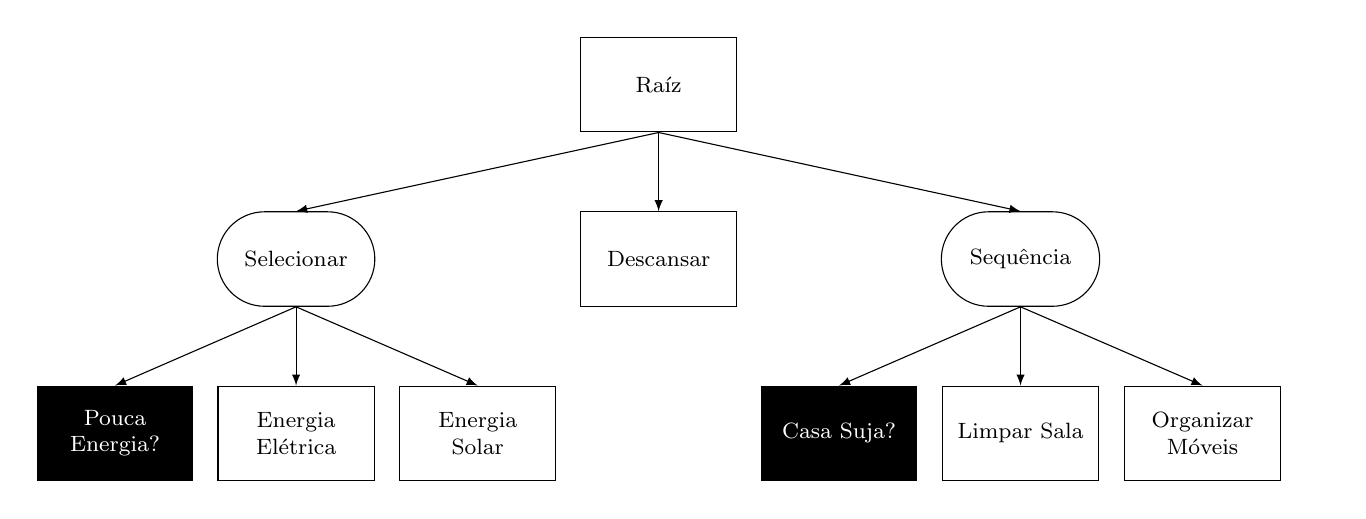
\begin{tikzpicture}[
    every node/.style={
        font=\footnotesize
    },
    composite/.style={
        minimum width=1.75cm, minimum height=1.2cm,
        text width=1.75cm,
        text centered,
        rounded rectangle,
        draw
    },
    action/.style={
        minimum width=1.75cm, minimum height=1.2cm,
        text width=1.75cm,
        text centered,
        rectangle,
        draw
    },
    precond/.style={
        minimum width=1.75cm, minimum height=1.2cm,
        text width=1.75cm,
        text centered,
        rectangle,
        fill=black,
        text=white
    }
]
\matrix [row sep=1cm, column sep=0.3cm] {
                                                &
                                                &
                                                &
    \node (n1)  [action]    {Raíz};             &
                                                &
                                                &
                                                &
    \\
                                                &
    \node (n2)  [composite] {Selecionar};       &
                                                &
    \node (n3)  [action]    {Descansar};        &
                                                &
    \node (n4)  [composite] {Sequência};        &
                                                &
                                                &
    \\
    \node (n5)  [precond]   {Pouca Energia?};   &
    \node (n6)  [action]    {Energia Elétrica}; &
    \node (n7)  [action]    {Energia Solar};    &
                                                &
    \node (n8)  [precond]   {Casa Suja?};       &
    \node (n9)  [action]    {Limpar Sala};      &
    \node (n10) [action]    {Organizar Móveis}; &
    \\
};
\draw[->,>=latex] (n1.south) -- (n2.north);
\draw[->,>=latex] (n1.south) -- (n3.north);
\draw[->,>=latex] (n1.south) -- (n4.north);

\draw[->,>=latex] (n2.south) -- (n5.north);
\draw[->,>=latex] (n2.south) -- (n6.north);
\draw[->,>=latex] (n2.south) -- (n7.north);

\draw[->,>=latex] (n4.south) -- (n8.north);
\draw[->,>=latex] (n4.south) -- (n9.north);
\draw[->,>=latex] (n4.south) -- (n10.north);
\end{tikzpicture}
\caption {\label{fig:behavior-tree-example}Exemplo de uma \textit{behaviour
tree} para representar um agente que deve carregar suas baterias caso seja
necessário, além de limpar e organizar a casa, descansando caso contrário.}
\end{figure}

Existem algumas outras técnicas que resolvem o mesmo problema que as
\textit{Behavior Trees} como, por exemplo, as \textbf{\textit{Finite State
Machines}} (máquinas de estados finitos), que são muito utilizadas em
inteligência artificial para jogos. Uma \textit{FSM} contém \textbf{estados} que
são ligados através de \textbf{transições}. Contudo, existem diversos problemas
com esta abordagem. A quantidade de estados e transições cresce
exponencialmente, os estados não podem ser reutilizados com facilidade e devemos
nos preocupar constantemente se existem transições inválidas no modelo. As
\textit{FSMs} possuem, resumidamente, um problema de modularidade.

Outra técnica muito utilizada são as \textbf{\textit{Hierarchical Finite State
Machines}} (máquinas de estados finitos hierárquicas). O objetivo da criação
desta técnica foi justamente mitigar alguns dos problemas das \textit{FSMs},
permitindo o englobamento de estados em uma hierarquia. Entretanto, o problema
de extensibilidade e praticidade ainda existem, porque ainda é baseada em
transições.


%----------
\section{\label{section:neat}NEAT}
% NEAT
% neuroevolução
% NEAT evolui os pesos e a rede em sí (TWEANNs)
% representação genética da rede
% problemas comuns em TWEANNs que o NEAT resolve
% (competing conventions, protecting innovation e initial population)

\begin{mdframed}[backgroundcolor=green!20]
\begin{itemize}
    \item
        Introdução: Escolha da técnica, história, paper
    \item
        Relação com aprendizado de máquina
    \item
        Relação com algoritmos genéticos
    \item
        Relação com redes neurais
    \item
        Explicação sobre a técnica: detalhamento de como funciona, termos
        técnicos, exemplos, pedaços de código (se necessário)
    \item
        Como será utilizada na construção dos \textit{bots}
\end{itemize}
\end{mdframed}

\chapter{\label{chap:related-work}Trabalhos Relacionados}
% MarI/O
% - https://www.youtube.com/watch?v=qv6UVOQ0F44 
% - https://www.youtube.com/watch?v=iakFfOmanJU 
% - https://www.youtube.com/watch?v=S9Y_I9vY8Qw 

% Atari DeepMind
% - http://arxiv.org/pdf/1312.5602v1.pdf  

% NERO
% - http://nn.cs.utexas.edu/?stanley:ieeetec05 

\section{N.E.R.O: Neuro-Evolving Robotic Operatives}

\begin{mdframed}[backgroundcolor=green!20]
\begin{itemize}
    \item
        O que é
    \item
        Técnica utilizada (citar paper)
    \item
        Relevância com o nosso trabalho
\end{itemize}
\end{mdframed}

%----------
\section{Playing Atari with Deep Reinforcement Learning}
O artigo apresenta um modelo de \textit{deep learning} capaz de aprender
políticas de controle para sete jogos do \textit{console} Atari 2600, criando
uma inteligência artificial capaz de jogar eficientemente todos os jogos,
inclusive superando jogadores humanos em alguns deles. O modelo utiliza
aprendizado por reforço e uma rede neural convolucional treinada com um variante
de \textit{Q-learning} para criar o agente.

Para criar estas políticas de controle, os autores utilizaram uma plataforma de
testes de inteligência artificial chamada \textit{Arcade Learning Environment}.
A cada passo de execução, o agente interage com o emulador, recebendo
informações do estado do jogo e enviando os comandos que deseja executar. As
informações recebidas eram um vetor dos \textit{pixels} apresentados na tela, o
conjunto de de ações possíveis para o jogo em questão e um valor de recompensa
quando a pontuação do jogo era alterada.

Como as informações do estado do jogo eram altamente dimensionais -- 33600
\textit{pixels} de informação visual --, foi necessário realizar um
pré-processamento para reduzir a dimensionalidade do estado do jogo -- reduzindo
para 7600 \textit{pixels}. Mesmo com esta redução, as quantidade de informações
recebidas ainda era considerável. Por isto, a utilização de \textit{deep
learning} e redes neurais convolucionais provou ser uma excelente -- e
necessária -- escolha para realizar o treinamento do agente. Contudo, o
treinamento do agente utilizando esta técnica é extremamente demorado.

Como a dimensionalidade do estado do jogo fornecido pela ferramenta
\textit{SpelunkBots} não é tão grande quanto a do trabalho em questão, optamos
por não fazer uso de \textit{deep learning}, mesmo que a técnica também seja
muito promissora.


%----------
\section{MarI/O}

Em junho de 2015, o canal do \textit{YouTube}
SethBling\footnote{https://www.youtube.com/user/sethbling/about} -- conhecido
por publicar vídeos de modificações de jogos como Mario e Minecraft -- divulgou
o vídeo \textit{MarI/O - Machine Learning for Video
Games}\footnote{https://www.youtube.com/watch?v=qv6UVOQ0F44}, que mostra um
jogador muito habilidoso completando o nível \textit{Donut Plains 1} de
\textit{Super Mario World}. É explicado, então, que o jogador em questão não é
humano, mas sim um programa de computador. Utilizando um emulador de
\textit{consoles} chamado
\textit{BizHawk}\footnote{http://tasvideos.org/BizHawk.html}, a linguagem de
programação \textit{Lua} e uma técnica de inteligência artificial chamada
\textit{\textbf{N.E.A.T}} (\textit{NeuroEvolution of Augmenting Topologies})
\cite{stanley:ec02} -- explicada detalhadamente no capítulo \ref{chap:neat} --,
o autor programou um \textit{bot} capaz de aprender como jogar o nível em
questão do início ao fim com sucesso. Como é explicado no vídeo, inicialmente o
\textit{bot} não conhecia absolutamente nada sobre como jogar \textit{Super
Mario World}. Contudo, através de várias simulações, adquiriu o conhecimento
necessário para superar todos os obstáculos presentes no nível.

\begin{figure}[htb!]
\centering
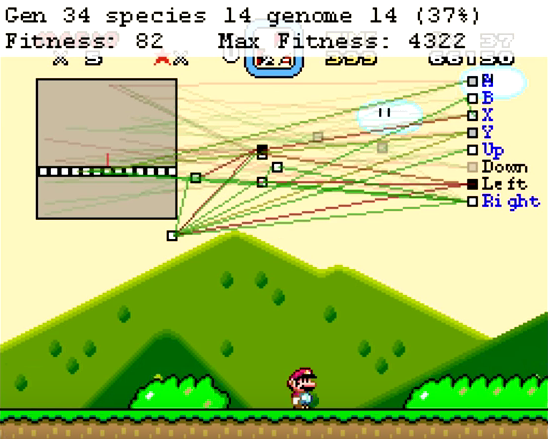
\includegraphics[width=.65\textwidth]{fig/mar-io-example.png}
\caption{\label{fig:mar-io-example}Exemplo da visão do jogo \textit{Super
Mario World} através do projeto \textit{MarI/O}, mostrando elementos de
controle usados pelo NEAT, como a rede neural, as possíveis ações, as
gerações, as espécies, os genomas, entre outros.}
\end{figure}

Depois do sucesso no nível \textit{Donut Plains 1}, o autor realizou mais
experimentos da aplicação da técnica
\textit{NEAT}\footnote{https://www.youtube.com/watch?v=iakFfOmanJU}
\footnote{https://www.youtube.com/watch?v=S9Y\_I9vY8Qw}. Inicialmente, testou em
dois outros níveis de \textit{Super Mario World}. Em \textit{Donut Plains 4}, o
processo de aprendizagem foi complicado, pois para obter progresso no nível era
necessário que aprendesse a interagir com certos elementos do mapa, e o autor
decidiu abortar o processo de aprendizagem. Já em \textit{Yoshi's Island 1},
obteve sucesso e foi capaz de concluir o nível. Com os testes finalizados, o
autor decidiu aplicar a técnica em outros dois jogos da franquia \textit{Mario}.
Em \textit{Super Mario Bros}, o \textit{bot} concluiu o primeiro nível e,
surpreendentemente, foi capaz de descobrir um \textit{glitch} no jogo que o
permitia passar por um segmento do segundo nível com maior rapidez. Em
\textit{Super Mario Kart}, depois de receber treinamento, o \textit{bot} foi
capaz de terminar uma corrida no nível \textit{Mario Circuit 1} em primeiro
lugar contra outros jogadores controlados pelo computador -- na dificuldade mais
fácil do jogo.

O \textit{MarI/O} é especialmente interessante e relevante porque tem um
objetivo muito similar ao deste trabalho: criar uma inteligência artificial
capaz de jogar uma partida de um jogo. Contudo, nos jogos escolhidos por
SethBling, os níveis são sempre os mesmos, o que torna mais fácil medir o
desempenho de um \textit{bot}, pois a disposição do nível é sempre igual e o
objetivo final sempre se encontra no mesmo lugar. Este não é o caso em
\textit{Spelunky}, onde os níveis são gerados proceduralmente. Além disso, os
níveis de \textit{Super Mario World} e \textit{Super Mario Bros.} são
essencialmente horizontais, e movimentar o personagem para a direita quase
sempre garante alguma forma de progresso. Isto facilita ainda mais o processo de
treinamento dos \textit{bots}. Em \textit{Spelunky} não é possível saber de
antemão onde se encontra a saída do nível e o movimento horizontal não garante o
progresso, visto que os níveis não são essencialmente horizontais. Estes fatores
influenciam na dificuldade de realizar o treinamento dos \textit{bots}.

\chapter{\label{chap:project}Projeto}
O primeiro passo para dar início ao desenvolvimento deste projeto é obter uma
cópia do projeto \textit{SpelunkBots}, hospedada no \textit{website} de
versionamento de código
\textit{GitHub}\footnote{https://github.com/GET-TUDA-CHOPPA/SpelunkBots}. O
\textit{framework} conta com o código modificado do \textit{Spelunky} e uma
distribuição do \textit{GameMaker Pro 8.0}, utilizada para compilar e executar o
jogo.

Conforme detalhado na seção \ref{section:spelunkbots}, o \textit{SpelunkBots}
disponibiliza duas opções de linguagem de programação para realizar o
desenvolvimento dos \textit{bots}: \textit{GML} ou C++. Portanto, a próxima
etapa do projeto é definir a linguagem de programação que vamos utilizar. Para
este projeto, escolhemos a linguagem de programação \textbf{C++}, tendo em vista
que o desenvolvimento utilizando a linguagem \textit{GML} é limitado. Além
disso, C++ é uma linguagem amadurecida e possui bibliotecas que implementam
\textit{NEAT}\footnote{http://nn.cs.utexas.edu/?neat-c} e \textit{Behavior
Trees}\footnote{https://github.com/aigamedev/bts}. O uso dessas bibliotecas
salva tempo de desenvolvimento e permite que o foco do trabalho seja somente nos
\textit{bots}, e não na arquitetura necessária.

Sabendo que a técnica \textit{NEAT} requer que o \textit{bot} receba treinamento
através de diversas simulações do jogo, optamos pelo uso de um servidor
dedicado, pois este processo pode ser demorado e executar o processo de
treinamento em uma máquina doméstica -- que está muito mais sujeita a ser
desligada acidentalmente ou intencionalmente -- é arriscado. O servidor em
questão utiliza um sistema operacional baseado em \textit{Linux}.  Contudo,
\textit{Spelunky} foi desenvolvido utilizando uma versão muito antiga do
\textit{GameMaker}, que só pode ser executada no sistema operacional
\textit{Windows}, e o \textit{SpelunkBots} utiliza um projeto em \textit{Visual
Studio} para realizar a compilação do código externo dos \textit{bots}. Como
nosso servidor é baseado em \textit{Linux}, é necessário realizar algumas
adaptações no processo de compilação. Assim, utilizaremos o \textit{software}
\textit{Wine}\footnote{https://winehq.org}, que nos permitirá executar programas
da plataforma \textit{Windows} dentro do sistema operacional \textit{Linux}, e o
\textit{software} \textit{MinGW}\footnote{http://www.mingw.org}, que realizará a
compilação do código C++ e a geração da \textit{DLL}.

O próximo passo é integrar as bibliotecas de inteligência artificial
selecionados com o projeto do \textit{SpelunkBots}, para que estejam incluídas
na solução \textit{DLL}. Ao concluir este passo, as configurações necessárias de
projeto estarão finalizadas, e daremos início ao desenvolvimento dos
\textit{bots}.


\section{Desenvolvimento dos \textit{bots}}
O \textit{framework} \textit{SpelunkBots} provê uma interface comum para o
desenvolvimento dos \textit{bots} em C++, chamada \textbf{\textit{IBot.h}}. Esta
interface é responsável por expor os métodos e variáveis que os \textit{bots}
utilizam para comunicar-se com o jogo. Portanto, qualquer código de \textit{bot}
desenvolvido deverá partir desta interface. Analisando o arquivo \textit{IBot.h}
é possível perceber que a interface obriga o desenvolvedor a implementar
\textbf{pelo menos} o método \textbf{\textit{Update}}, chamado em todas as
etapas de execução do \textit{bot} para receber informações e enviar comandos ao
jogo. Existem dois outros métodos que podem ser úteis ao desenvolvedor, mas que
não possuem obrigatoriedade de implementação:

\begin{itemize}
	\item
		\textbf{\textit{Reset}:} chamada no início de todas as etapas de
		execução do \textit{bot} para reiniciar todas as suas variáveis de
		controle. Possui uma implementação padrão que reinicia apenas as
		variáveis essenciais (esquerda, direita, pular e atacar).

	\item
		\textbf{\textit{NewLevel}:} chamada toda vez que o \textit{bot} entra em
		um novo nível. Pode ser usada para descartar informações do nível
		anterior sem que seja necessário reiniciar todas as variáveis do
		\textit{bot}. Na implementação padrão, não executa nada.
\end{itemize}

Uma implementação mínima de um \textit{bot} utilizando a interface
\textit{IBot.h} necessitaria, portanto, de dois arquivos: um arquivo
\textit{header}, que conterá as declarações dos métodos e variáveis a serem
utilizadas -- ilustrado na Figura \ref{alg:project-example-bot-header} --, e
um arquivo de implementação -- ilustrado na Figura
\ref{alg:project-example-bot-impl} --, que conterá a implementação das funções
descritas no arquivo \textit{header}.

\begin{algorithm}[H]
\lstinputlisting[language=c++]{code/ExampleBot.h}
\caption[Definição de métodos e variáveis de um \textit{bot} de exemplo.]
{\label{alg:project-example-bot-header}Definição de métodos e variáveis de um
\textit{bot} de exemplo.}
\end{algorithm}

\begin{algorithm}[H]
\lstinputlisting[language=c++]{code/ExampleBot.cpp}
\caption[Implementação dos métodos e variáveis de um \textit{bot} de exemplo.]
{\label{alg:project-example-bot-impl}Implementação dos métodos e variáveis de um
\textit{bot} de exemplo.}
\end{algorithm}

É importante ressaltar que, devido ao processo de \textbf{treinamento} do
\textit{bot} que faz uso da técnica \textit{NEAT}, temos a necessidade realizar
operações de \textbf{leitura} e \textbf{escrita} de arquivos, portanto, é
interessante definir um tipo de \textit{bot} que comporte tais operações. Dessa
forma, além do método \textit{Update}, implementaremos os métodos
\textbf{\textit{ReadTrainingData}} e \textbf{\textit{SaveTrainingData}}.

\chapter{\label{chap:work-plan}Etapas de Desenvolvimento}
Para se obter um maior detalhamento do que será desenvolvido durante a execução
deste trabalho, analisamos os objetivos gerais deste trabalho, citados no
capítulo \ref{chap:problem-objectives}, e os elementos de projeto necessários,
mencionados no capítulo \ref{chap:project}, para definir as \textbf{atividades}
serão executadas ao longo deste trabalho:

\begin{enumerate}
	\item
		Obter uma cópia do \textit{framework} \textit{SpelunkBots}
	\item
		Realizar modificações no \textit{SpelunkBots} para que possa ser
		executado na plataforma \textit{Linux}
	\item
		Buscar por bibliotecas auxiliares para o uso da técnica \textit{NEAT}
	\item
		Buscar por bibliotecas auxiliares para o uso da técnica \textit{Behavior
		Trees}
	\item
		Realizar as configurações da ferramenta \textit{SpelunkBots} para
		permitir o desenvolvimento de \textit{bots} utilizando \textit{Behavior
		Trees}
	\item
		Desenvolver um \textit{bot} utilizando \textit{Behavior Trees}
	\item
		Coletar dados da execução do \textit{bot} baseado em \textit{Behavior
		Trees} em uma série de mapas pré-estabelecidos e aleatórios
	\item
		Realizar as configurações da ferramenta \textit{SpelunkBots} para
		permitir o desenvolvimento de \textit{bots} utilizando \textit{NEAT}
	\item
		Desenvolver um \textit{bot} utilizando \textit{NEAT}
	\item
		Coletar dados da execução do \textit{bot} baseado em \textit{NEAT} em
		uma série de mapas pré-estabelecidos e aleatórios
	\item
		Analisar e comparar os resultados obtidos entre os \textit{bots}
		baseados em \textit{Behavior Trees} e \textit{NEAT}
\end{enumerate}

A metodologia de desenvolvimento adotada para este trabalho é iterativa e
incremental, particionada em iterações de uma semana, onde serão desenvolvidas
uma ou mais atividades. A tabela \ref{tab:work-plan} ilustra o cronograma
definido para a segunda etapa deste trabalho, baseado nas atividades definidas
anteriormente.

\begin{table}[H]
\centering
\caption{Objetivos por Iteração}
\label{tab:work-plan}
\begin{tabular}{c|c|c|c|c|c|c|c|c|c|c|c|c|c|c|c|}
\cline{2-16}
{\bf}                                 & \multicolumn{3}{c|}{{\bf Ago/16}} & \multicolumn{4}{c|}{{\bf Set/16}}     & \multicolumn{4}{c|}{{\bf Out/16}}      & \multicolumn{4}{c|}{{\bf Nov/16}}     \\ \hline
\multicolumn{1}{|c|}{{\bf Atividade}} & {\bf 1} & {\bf 2} & {\bf 3}	      & {\bf 4} & {\bf 5} & {\bf 6} & {\bf 7} & {\bf 8} & {\bf 9} & {\bf 10} & \bf{11} & \bf{12} & \bf{13} & \bf{14} & \bf{15} \\ \hline
\multicolumn{1}{|c|}{{\bf 1}}         & X       &         &               &         &         &         &         &         &         &          &         &         &         &         &         \\ \hline
\multicolumn{1}{|c|}{{\bf 2}}         & X       &         &               &         &         &         &         &         &         &          &         &         &         &         &         \\ \hline
\multicolumn{1}{|c|}{{\bf 3}}         &         & X       &               &         &         &         &         &         &         &          &         &         &         &         &         \\ \hline
\multicolumn{1}{|c|}{{\bf 4}}         &         &         & X             &         &         &         &         &         &         &          &         &         &         &         &         \\ \hline
\multicolumn{1}{|c|}{{\bf 5}}         &         &         &               & X       &         &         &         &         &         &          &         &         &         &         &         \\ \hline
\multicolumn{1}{|c|}{{\bf 6}}         &         &         &               &         & X       & X       & X       &         &         &          &         &         &         &         &         \\ \hline
\multicolumn{1}{|c|}{{\bf 7}}         &         &         &               &         &         &         &         & X       &         &          &         &         &         &         &         \\ \hline
\multicolumn{1}{|c|}{{\bf 8}}         &         &         &               &         &         &         &         &         & X       &          &         &         &         &         &         \\ \hline
\multicolumn{1}{|c|}{{\bf 9}}         &         &         &               &         &         &         &         &         &         & X        & X       & X       &         &         &         \\ \hline
\multicolumn{1}{|c|}{{\bf 10}}        &         &         &               &         &         &         &         &         &         &          &         &         & X       &         &         \\ \hline
\multicolumn{1}{|c|}{{\bf 11}}        &         &         &               &         &         &         &         &         &         &          &         &         &         & X       & X       \\ \hline
\end{tabular}
\end{table}

\section{Detalhamento das Atividades}
Esta seção detalha brevemente o que será desenvolvido em cada atividade do
trabalho, bem como a relação de data de início e término.

\begin{enumerate}
    \item
        Obter uma cópia do SpelunkBots
    \begin{description}[leftmargin=!,labelwidth=\widthof{\bfseries Descrição}]
        \item [Descrição]
            Para possibilitar o desenvolvimento desse trabalho, preciamos obter
            uma cópia do projeto SpelunkyBots, permitindo então que façamos o
            desenvolvimento de \textit{bots} utilizando esse \textit{framework}.
        \item [Iterações]
            1
        \item [Período]
            01/08/2016 - 08/08/2016
    \end{description}

    \item
		Realizar modificações no \textit{SpelunkBots} para que possa ser
		executado na plataforma \textit{Linux}
    \begin{description}[leftmargin=!,labelwidth=\widthof{\bfseries Descrição}]
        \item [Descrição]
            O SpelunkBots não possui uma distribuição para Linux. Como vamos
            utilizar um servidor para o treinamento dos \textit{bots},
            precisamos fazer adaptações para que o jogo funcione nessa
            plataforma.
        \item [Iterações]
            1
        \item [Período]
            08/08/2016 - 15/08/2016
    \end{description}

    \item
        Buscar por bibliotecas auxiliares para o uso da técnica \textit{NEAT}
    \begin{description}[leftmargin=!,labelwidth=\widthof{\bfseries Descrição}]
        \item [Descrição]
            O uso de bibliotecas acelera o desenvolvimento da aplicação. Dessa
            forma, devemos buscar uma biblioteca para o uso de \textit{NEAT}.
            Caso encontremos tal biblioteca, é necessário ver se a mesma pode
            ser usada no nosso projeto.
        \item [Iterações]
            2
        \item [Período]
            15/08/2016 - 22/08/2016
    \end{description}

    \item
        Buscar por bibliotecas auxiliares para o uso da técnica
        \textit{Behavior Trees}
    \begin{description}[leftmargin=!,labelwidth=\widthof{\bfseries Descrição}]
        \item [Descrição]
            O uso de bibliotecas acelera o desenvolvimento da aplicação. Dessa
            forma, devemos buscar uma biblioteca para o uso de \textit{behavior
            trees}.  Caso encontremos tal biblioteca, é necessário ver se a
            mesma pode
            ser usada no nosso projeto.
        \item [Iterações]
            3
        \item [Período]
            22/08/2016 - 05/09/2016
    \end{description}

	\item
		Realizar as configurações da ferramenta \textit{SpelunkBots} para
		permitir o desenvolvimento de \textit{bots} utilizando \textit{Behavior
		Trees}
    \begin{description}[leftmargin=!,labelwidth=\widthof{\bfseries Descrição}]
        \item [Descrição]
            Devemos estudar como utilizar as bibliotecas de \textit{Behavior
            Trees} encontradas para integrá-las ao código do
            \textit{SpelunkBots}, modificando ou incrementando o código
            existente.
        \item [Iterações]
            4
        \item [Período]
            05/09/2016 - 12/09/2016
    \end{description}
	\item
		Desenvolver um \textit{bot} utilizando \textit{Behavior Trees}
    \begin{description}[leftmargin=!,labelwidth=\widthof{\bfseries Descrição}]
        \item [Descrição]
            Desenvolvimento do código do \textit{bot} que fará uso da técnica
            \textit{Behavior Trees}.
        \item [Iterações]
            5, 6 e 7
        \item [Período]
            12/09/2016 - 03/10/2016
    \end{description}
	\item
		Coletar dados da execução do \textit{bot} baseado em \textit{Behavior
		Trees} em uma série de mapas pré-estabelecidos e aleatórios
    \begin{description}[leftmargin=!,labelwidth=\widthof{\bfseries Descrição}]
        \item [Descrição]
            Coletar dados de execução, exportando os resultados obtidos,
            permitindo que sejam feitas análises sobre o \textit{bot}
            utilizando esses dados.
        \item [Iterações]
            8
        \item [Período]
            03/10/2016 - 10/10/2016
    \end{description}
	\item
		Realizar as configurações da ferramenta \textit{SpelunkBots} para
		permitir o desenvolvimento de \textit{bots} utilizando \textit{NEAT}
    \begin{description}[leftmargin=!,labelwidth=\widthof{\bfseries Descrição}]
        \item [Descrição]
            Devemos estudar como utilizar as bibliotecas de textit{NEAT}
            encontradas para integrá-las ao código do \textit{SpelunkBots},
            modificando ou incrementando o código existente.
        \item [Iterações]
            9
        \item [Período]
            10/10/2016 - 17/10/2016
    \end{description}
	\item
		Desenvolver um \textit{bot} utilizando \textit{NEAT}
    \begin{description}[leftmargin=!,labelwidth=\widthof{\bfseries Descrição}]
        \item [Descrição]
            Desenvolvimento do código do \textit{bot} que fará uso da técnica
            \textit{NEAT}.
        \item [Iterações]
            10, 11 e 12
        \item [Período]
            17/10/2016 - 07/11/2016
    \end{description}
	\item
		Coletar dados da execução do \textit{bot} baseado em \textit{NEAT} em
		uma série de mapas pré-estabelecidos e aleatórios
    \begin{description}[leftmargin=!,labelwidth=\widthof{\bfseries Descrição}]
        \item [Descrição]
            Coletar dados de execução, exportando os resultados obtidos,
            permitindo que sejam feitas análises sobre o \textit{bot}
            utilizando esses dados.
        \item [Iterações]
            13
        \item [Período]
            07/11/2016 - 14/11/2016
    \end{description}
	\item
		Analisar e comparar os resultados obtidos entre os \textit{bots}
		baseados em \textit{Behavior Trees} e \textit{NEAT}
    \begin{description}[leftmargin=!,labelwidth=\widthof{\bfseries Descrição}]
        \item [Descrição]
            Devemos analisar o uso das técnicas escolhidas nesse trabalho,
            verificando o desempenho delas para a solução do problema.
        \item [Iterações]
            14 e 15
        \item [Período]
            14/11/2016 - 28/11/2016
    \end{description}
\end{enumerate}


\appendix
\chapter{\label{appendix:spelunkbots-variables}Lista de Variáveis Globais
de SpelunkBots}

\section{Movimentação do \textit{Bot}}
Estas são as variáveis \textit{booleanas} utilizadas para controlar quais botões
devem ser pressionados a cada etapa de execução, indicando aos \textit{bots}
quais ações devem executar:

\begin{center}
    \begin{tabular}{ |c| }
        \hline
        \textbf{Variável} \\ \hline
        global.attack \\ \hline
        global.duck \\ \hline
        global.goLeft \\ \hline
        global.goRight \\ \hline
        global.jump \\ \hline
        global.lookUp \\ \hline
        global.payp \\ \hline
        global.running \\ \hline
    \end{tabular}
\end{center}

\section{Tipo do Terreno}
Valores possíveis para os nodos de um mapa de \textit{Spelunky}:

\begin{center}
    \begin{tabular}{ |c|c| }
        \hline
        \textbf{Variável} & \textbf{Valor} \\ \hline
        global.spEmptyNode & 0 \\ \hline
        global.spStandardTerrain & 1 \\ \hline
        global.spLadder & 2 \\ \hline
        global.spEntrance & 3 \\ \hline
        global.spExit & 4 \\ \hline
        global.spSacAlter & 5 \\ \hline
        global.spArrowTrapRight & 6 \\ \hline
        global.spArrowTrapLeft & 7 \\ \hline
        global.spIsInShop & 8 \\ \hline
        global.spIce & 9 \\ \hline
        global.spSpike & 10 \\ \hline
        global.spSpearTrap & 11 \\ \hline
    \end{tabular}
\end{center}

\section{Inimigos e Armadilhas}
De modo similar aos valores de terreno, cada tipo de inimigo e armadilha possui
um valor de representação:

\begin{center}
    \begin{tabular}{ |c|c| }
        \hline
        \textbf{Variável} & \textbf{Valor} \\ \hline
        global.spGhost & 1 \\ \hline
        global.spBat & 2 \\ \hline
        global.spScarab & 3 \\ \hline
        global.spSpider & 4 \\ \hline
        global.spGiantSpiderHang & 5 \\ \hline
        global.spGiantSpider & 6 \\ \hline
        global.spFrog & 7 \\ \hline
        global.spFireFrog & 8 \\ \hline
        global.spZombie & 9 \\ \hline
        global.spVampire & 10 \\ \hline
        global.spPiranha & 11 \\ \hline
        global.spJaws & 12 \\ \hline
        global.spDeadFish & 13 \\ \hline
        global.spManTrap & 14 \\ \hline
        global.spMonkey & 15 \\ \hline
        global.spYeti & 16 \\ \hline
        global.spYetiKing & 17 \\ \hline
        global.spUFO & 18 \\ \hline
        global.spUFOCrash & 19 \\ \hline
        global.spAlienEject & 20 \\ \hline
        global.spAlien & 21 \\ \hline
        global.spAlienBoss & 22 \\ \hline
        global.spBarrierEmitter & 23 \\ \hline
        global.spBarrier & 24 \\ \hline
        global.spCaveman & 25 \\ \hline
        global.spHawkman & 26 \\ \hline
        global.spMagma & 27 \\ \hline
        global.spMagmaTrail & 28 \\ \hline
        global.spMagmaMan & 29 \\ \hline
        global.spTombLord & 30 \\ \hline
    \end{tabular}
\end{center}

\begin{center}
    \begin{tabular}{ |c|c| }
        \hline
        global.spOlmec & 31 \\ \hline
        global.spCavemanWorship & 32 \\ \hline
        global.spHawkmanWorship & 33 \\ \hline
        global.spOlmecDebris & 34 \\ \hline
        global.spSnake & 35 \\ \hline
        global.spSpiderHang & 36 \\ \hline
        global.spMagmaMan & 37 \\ \hline
        global.spShopkeeper & 38 \\ \hline
        global.spBones & 60 \\ \hline
        global.spSmashTrap & 61 \\ \hline
        global.spCeilingTrap & 62 \\ \hline
        global.spBoulder & 63 \\ \hline
        global.spSpringTrap & 99 \\ \hline
    \end{tabular}
\end{center}

\section{Objetos}
Existem diversos objetos em \textit{Spelunky} com os quais o jogador pode
interagir, e cada objeto é representado por um valor:

\begin{center}
    \begin{tabular}{ |c|c| }
        \hline
        \textbf{Variável} & \textbf{Valor} \\ \hline
        global.spGoldBar & 1 \\ \hline
        global.spGoldBars & 2 \\ \hline
        global.spEmerald & 3 \\ \hline
        global.spEmeraldBig & 4 \\ \hline
        global.spSapphire & 5 \\ \hline
        global.spSapphireBig & 6 \\ \hline
        global.spRuby & 7 \\ \hline
        global.spRubyBig & 8 \\ \hline
        global.spDiamond & 9 \\ \hline
        global.spGoldNugget & 10 \\ \hline
        global.spGoldChunk & 11 \\ \hline
        global.spChest & 12 \\ \hline
        global.spLockedChest & 13 \\ \hline
        global.spKey & 14 \\ \hline
        global.spCrate & 15 \\ \hline
        global.spFlareCrate & 16 \\ \hline
        global.spBombBag & 17 \\ \hline
        global.spBombBox & 18 \\ \hline
        global.spPaste & 19 \\ \hline
        global.spRopePile & 20 \\ \hline
        global.spParachute & 21 \\ \hline
        global.spCompass & 22 \\ \hline
        global.spSpringShoes & 23 \\ \hline
        global.spSpikeShoes & 24 \\ \hline
        global.spJordans & 25 \\ \hline
        global.spSpecs & 26 \\ \hline
        global.spUdjat & 27 \\ \hline
        global.spCrown & 28 \\ \hline
        global.spKapala & 29 \\ \hline
        global.spAnkh & 30 \\ \hline
        global.spGloves & 31 \\ \hline
        global.spMitt & 32 \\ \hline
        global.spJetpack & 33 \\ \hline
        global.spCape & 34 \\ \hline
        global.spRopeBag & 35 \\ \hline
    \end{tabular}
\end{center}

\section{Dados do Jogador}
Em adição às variáveis de controle, as variáveis de dados do jogador são
utilizadas para auxiliar o desenvolvedor a implementar o comportamento de um
\textit{bot}.

\begin{center}
    \begin{tabular}{ |c| }
        \hline
        \textbf{Variável (boolean)} \\ \hline
        global.hasGoal \\ \hline
        global.spIsInAir \\ \hline
        global.spIsJetpacking \\ \hline
        global.spJumpPressedPreviously \\ \hline
        global.itemGoal \\ \hline
        global.fogGoal \\ \hline
        global.endGoal \\ \hline
        global.headingRight \\ \hline
        global.headingLeft \\ \hline
        global.isPlayerHanging \\ \hline
        global.isPlayerHodldingHoldenIdol \\ \hline
    \end{tabular}
\end{center}

\begin{center}
    \begin{tabular}{ |c| }
        \hline
        \textbf{Variável (número inteiro)} \\ \hline
        global.playerPositionX \\ \hline
        global.playerPositionY \\ \hline
        global.playerPositionXNode \\ \hline
        global.playerPositionYNode \\ \hline
        global.pathCount \\ \hline
        global.tempID \\ \hline
        global.waitTimer \\ \hline
    \end{tabular}
\end{center}

\chapter{\label{appendix:spelunky-details}Detalhamento dos Obstáculos e
Itens em Spelunky}

\section{\label{section:spelunky-traps}Armadilhas}

\begin{description}
    \item[Espinhos]
    \item[Lança flechas]
    \item[Pedregulho]
    \item[Armadilha \textit{tiki}]
    \item[Trampolim]
    \item[Campo de força]
    \item[Pedra de esmagar]
    \item[Teto com espinhos]
    \item[Lava]
    \item[Teia de aranha]
    \item[Abismo]
    \item[Gelo fino]
    \item[Baú falso]
    \item[Vaso com monstros]
\end{description}

\section{\label{section:spelunky-monsters}Monstros}

\begin{description}
    \item[Comerciante]
    \item[Cobra]
    \item[Morcego]
    \item[Aranha]
    \item[Aranha gigante]
    \item[Esqueleto]
    \item[Homem da caverna]
    \item[Escaravelho]
    \item[Sapo]
    \item[Planta carnívora]
    \item[Piranha]
    \item[Macaco]
    \item[Jiang Shi]
    \item[Vampiro]
    \item[Fantasma]
    \item[Yeti]
    \item[Rei Yeti]
    \item[Alien]
    \item[OVNI]
    \item[Rei alien]
    \item[Homem águia]
    \item[Homem magma]
    \item[Múmia]
    \item[Olmec]
\end{description}

\section{\label{section:spelunky-items}Itens}

\begin{description}
    \item[Corda]
    \item[Bomba]
    \item[Paraquedas]
    \item[Compasso]
    \item[Luva de escalar]
    \item[Luva de arremessar]
    \item[Bota com mola]
    \item[Bota com espinhos]
    \item[Cola para bombas]
    \item[Óculos]
    \item[Picareta]
    \item[Machete]
    \item[Arco]
    \item[Pistola]
    \item[Pistola]
    \item[Espingarda]
    \item[Arma de teia]
    \item[Capa]
    \item[Mochila à jato]
    \item[Labareda]
    \item[Caixa de labaredas]
    \item[Udjat Eye]
    \item[Ankh]
    \item[Hedjet]
    \item[Sceptre]
    \item[Tesouro]
    \item[Ídolo dourado]
    \item[Caveira de cristal]
    \item[Ídolo dourado gigante]
    \item[Caixote]
    \item[Baú]
    \item[Baú grande]
    \item[Chave]
    \item[Pedra]
    \item[Vaso]
    \item[Flecha]
    \item[Caveira]
    \item[Esqueleto de piranha]
    \item[Cadáver]
    \item[Cabeça de picareta]
    \item[Lanterna]
    \item[Teletransportador]
    \item[Kapala]
    \item[Bola com corrente]
\end{description}


\bibliographystyle{tcc-num}
\bibliography{final-assignment-1-bib}

\end{document}
